\documentclass[9pt,a4paper,]{extarticle}

\usepackage{f1000_styles}

\usepackage[pdfborder={0 0 0}]{hyperref}

\usepackage[numbers]{natbib}
\bibliographystyle{unsrtnat}


%% maxwidth is the original width if it is less than linewidth
%% otherwise use linewidth (to make sure the graphics do not exceed the margin)
\makeatletter
\def\maxwidth{ %
  \ifdim\Gin@nat@width>\linewidth
    \linewidth
  \else
    \Gin@nat@width
  \fi
}
\makeatother

\usepackage{color}
\usepackage{fancyvrb}
\newcommand{\VerbBar}{|}
\newcommand{\VERB}{\Verb[commandchars=\\\{\}]}
\DefineVerbatimEnvironment{Highlighting}{Verbatim}{commandchars=\\\{\}}
% Add ',fontsize=\small' for more characters per line
\usepackage{framed}
\definecolor{shadecolor}{RGB}{248,248,248}
\newenvironment{Shaded}{\begin{snugshade}}{\end{snugshade}}
\newcommand{\AlertTok}[1]{\textcolor[rgb]{0.94,0.16,0.16}{#1}}
\newcommand{\AnnotationTok}[1]{\textcolor[rgb]{0.56,0.35,0.01}{\textbf{\textit{#1}}}}
\newcommand{\AttributeTok}[1]{\textcolor[rgb]{0.77,0.63,0.00}{#1}}
\newcommand{\BaseNTok}[1]{\textcolor[rgb]{0.00,0.00,0.81}{#1}}
\newcommand{\BuiltInTok}[1]{#1}
\newcommand{\CharTok}[1]{\textcolor[rgb]{0.31,0.60,0.02}{#1}}
\newcommand{\CommentTok}[1]{\textcolor[rgb]{0.56,0.35,0.01}{\textit{#1}}}
\newcommand{\CommentVarTok}[1]{\textcolor[rgb]{0.56,0.35,0.01}{\textbf{\textit{#1}}}}
\newcommand{\ConstantTok}[1]{\textcolor[rgb]{0.00,0.00,0.00}{#1}}
\newcommand{\ControlFlowTok}[1]{\textcolor[rgb]{0.13,0.29,0.53}{\textbf{#1}}}
\newcommand{\DataTypeTok}[1]{\textcolor[rgb]{0.13,0.29,0.53}{#1}}
\newcommand{\DecValTok}[1]{\textcolor[rgb]{0.00,0.00,0.81}{#1}}
\newcommand{\DocumentationTok}[1]{\textcolor[rgb]{0.56,0.35,0.01}{\textbf{\textit{#1}}}}
\newcommand{\ErrorTok}[1]{\textcolor[rgb]{0.64,0.00,0.00}{\textbf{#1}}}
\newcommand{\ExtensionTok}[1]{#1}
\newcommand{\FloatTok}[1]{\textcolor[rgb]{0.00,0.00,0.81}{#1}}
\newcommand{\FunctionTok}[1]{\textcolor[rgb]{0.00,0.00,0.00}{#1}}
\newcommand{\ImportTok}[1]{#1}
\newcommand{\InformationTok}[1]{\textcolor[rgb]{0.56,0.35,0.01}{\textbf{\textit{#1}}}}
\newcommand{\KeywordTok}[1]{\textcolor[rgb]{0.13,0.29,0.53}{\textbf{#1}}}
\newcommand{\NormalTok}[1]{#1}
\newcommand{\OperatorTok}[1]{\textcolor[rgb]{0.81,0.36,0.00}{\textbf{#1}}}
\newcommand{\OtherTok}[1]{\textcolor[rgb]{0.56,0.35,0.01}{#1}}
\newcommand{\PreprocessorTok}[1]{\textcolor[rgb]{0.56,0.35,0.01}{\textit{#1}}}
\newcommand{\RegionMarkerTok}[1]{#1}
\newcommand{\SpecialCharTok}[1]{\textcolor[rgb]{0.00,0.00,0.00}{#1}}
\newcommand{\SpecialStringTok}[1]{\textcolor[rgb]{0.31,0.60,0.02}{#1}}
\newcommand{\StringTok}[1]{\textcolor[rgb]{0.31,0.60,0.02}{#1}}
\newcommand{\VariableTok}[1]{\textcolor[rgb]{0.00,0.00,0.00}{#1}}
\newcommand{\VerbatimStringTok}[1]{\textcolor[rgb]{0.31,0.60,0.02}{#1}}
\newcommand{\WarningTok}[1]{\textcolor[rgb]{0.56,0.35,0.01}{\textbf{\textit{#1}}}}

% disable code chunks background
%\renewenvironment{Shaded}{}{}

% disable section numbers
\setcounter{secnumdepth}{0}

\setlength{\parindent}{0pt}
\setlength{\parskip}{6pt plus 2pt minus 1pt}



\begin{document}
\pagestyle{front}

\title{A Bioconductor workflow for the Bayesian analysis of spatial proteomics}

\author[1,2]{Oliver M. Crook}
\author[1]{Lisa M. Breckels}
\author[1]{Kathryn S. Lilley}
\author[2]{Paul D.W. Kirk}
\author[3]{Laurent Gatto\thanks{\ttfamily laurent.gatto@uclouvain.be}}
\affil[1]{Cambridge Centre for Proteomics, Department of Biochemistry, University of Cambridge, Cambridge, UK}
\affil[2]{MRC Biostatistics Unit, Cambridge Institute for Public Health, Cambridge, UK}
\affil[3]{de Duve Institute, UCLouvain, Brussels, Belgium}

\maketitle
\thispagestyle{front}

\begin{abstract}
Knowledge of the subcellular location of a protein gives valuable insight into its function. The field of spatial proteomics has become increasingly popular due to improved multiplexing capabilities in high-throughput mass-spectrometry, which have made it possible to systematically localise thousands of proteins per experiment. In parallel with these experimental advances, improved methods for analysing spatial proteomics data have also been developed. In this workflow, we demonstrate using \texttt{pRoloc} for the Bayesian analysis of spatial proteomics data. We detail the software infrastructure and then provide step-by-step guidance of the analysis, including setting up a pipeline, assessing convergence, and interpreting downstream results. In several places we provide additional details on Bayesian analysis to provide users with a holistic view of Bayesian analysis for spatial proteomics data.
\end{abstract}


\clearpage
\pagestyle{main}

\newcommand{\diag}{\mathop{\mathrm{diag}}}

\textbf{R version}: R version 3.5.2 Patched (2019-01-24 r76018)

\textbf{Bioconductor version}: 3.8

\hypertarget{introduction}{%
\section{Introduction}\label{introduction}}

Determining the the spatial subcellular distribution of
proteins enables novel insight into protein function
\citep{Crook:2018}. Many proteins function within a single location within the
cell, however it is estimated that up to half of the proteome is thought to
reside in mutiple locations, with some of these undergoing
dynamic relocalisation \citep{Thul:2017}. These phenomena lead
to variability and uncertainty in robustly assigning proteins to a unique
localisation. Functional
compartmentalisation of proteins allows the cell to control
biomolecular pathways and biochemical processes within the
cell. Therefore, proteins with multiple localisation may therefore have multiple
functional roles \citep{Jeffery:2009}. Machine learning algorithms that
fail to quantify uncertainty are unable to draw deeper insight into
understanding cell biology from mass-spectrometry (MS) based spatial
proteomics experiments. Hence, quantifying uncertainty allows us to
make rigorous assessments of protein subcellular localisation
and multi-localisation.

For proteins to carry out their functional role they must be localised
to the correct subcellular compartment, ensuring the biochemical conditions
for desired molecular interactions are met \citep{Gibson:2009}. Many
pathologies, including cancer and obesity are characterised by protein
mis-localisations \citep{Olkkonen:2006, Laurila:2009, Luheshi:2008, De:2011, Cody:2013, Kau:2004, Rodriguez:2004, Latorre:2005, Shin:2013, Siljee:2018}.
High-throughput spatial proteomics technologies have seen rapid improvement
over the last decade and now a single experiment can provide spatial information on
thousands of proteins at once \citep{Dunkley:2006, Foster:2006, hyper, DC:2018}.
As a result of these spatial proteomics technologies many biological systems have
been characterised \citep{Dunkley:2006, Tan:2009, Hall:2009, Breckels:2013, hyper, Thul:2017}.
The popularity of such methods is now evident with many new studies in recent years
\citep{hyper, Beltran:2016, Jadot:2017, Itzhak:2017, Mendes:2017, Hirst:2018, Davies:2018, Orre:2019, Nightingale:2019}.

Bayesian approaches to machine learning and statistics can
provide more insight, by providing uncertainty quantification
\citep{Gelman:1995}. In a parametric Bayesian setting, a parametric model
is proposed, along with a statement about our prior beliefs
of the model parameters. Bayes' theorem tells us how to update the
prior distribution of the parameters to obtain the posterior
distribution of the parameters after observing the data. It is the
posterior distribution which quantifies the uncertainty in the
parameters. This contrasts from a maximum-likelihood approach where we obtain only a
point estimate of the parameters.

Adopting a Bayesian framework for data analysis, though of much
interest to experimentalists, can be challenging. Once we have
specified a probabilistic model, computational approaches are typically used to obtain
the posterior distribution upon observation of the data. These
algorithms can have parameters that require tuning and a variety of settings, hindering
their practical use by those not familiar with Bayesian methodology. Even
once the algorithms have been correctly set-up, assessments of
convergence and guidance on how to interpret the results are often
sparse. This workflow presents a Bayesian analysis of spatial
proteomics to elucidate the process for practitioners. Our workflow also provides
a template for others interested in designing tools for the biological community
which rely on Bayesian inference.

Our model for the data is the t-augmented Gaussian mixture (TAGM)
model proposed in \citep{Crook:2018}. \citet{Crook:2018} provide a detailed
description of the model, rigorous comparisons and testing on many
spatial proteomics datasets, including a case study in which a hyperLOPIT
experiment is performed on mouse pluripotent stem cells
\citep{hyper, Mulvey:2017}. Revisiting these details is not the purpose of
this computational protocol; rather we present how to correctly use
the software and provide step-by-step guidance for interpreting the
results.

In brief, the TAGM model posits that each annotated sub-cellular niche
can be modelled using a Gaussian distribution. Thus the full complement
of proteins within the cell is captured as a mixture of Gaussians. The
highly dynamic nature of the cell means that many proteins are not
well captured by any of these multivariate Gaussian distributions, and
thus the model also includes an outlier component, which is mathematically
described as a multivariate student's t distribution. The heavy tails of
the t distribution allow it to better capture dispersed proteins.

There are two approaches to perform inference in the TAGM model. The
first, which we refer to as TAGM MAP, allows us to obtain \emph{maximum a
posteriori} estimates of posterior localisation probabilities; that
is, the modal posterior probability that a protein localises to that
class. This approach uses the expectation-maximisation (EM) algorithm
to perform inference \citep{EM:1977}. Whilst this is a interpretable
summary of the TAGM model, it only provides point estimates. For a
richer analysis, we also present a Markov-chain Monte-Carlo (MCMC) method
to perform fully Bayesian inference in our model, allowing us to
obtain full posterior localisation distributions. This method is
referred to as TAGM MCMC throughout the text.

This workflow begins with a brief review of some of the basic features
of mass spectrometry-based spatial proteomics data, including our
state-of-the-art computational infrastructure and bespoke software
suite. We then present each method in turn, detailing how to obtain
high quality results. We provide an extended discussion of the
TAGM MCMC method to highlight some of the challenges that may arise
when applying this method. This includes how to assess convergence of
MCMC methods, as well as methods for manipulating the output. We then
take the processed output and explain how to interpret the results, as
well as providing some tools for visualisation. We conclude with some
remarks and directions for the future.

\hypertarget{getting-started-and-infrastructure}{%
\section{Getting started and infrastructure}\label{getting-started-and-infrastructure}}

In this workflow, we are using version 1.23.2 of \texttt{pRoloc}
\citep{pRoloc:2014}. The package \texttt{pRoloc} contains algorithms and methods
for analysing spatial proteomics data, building on the \texttt{MSnSet}
structure provided in \texttt{MSnbase}. The \texttt{pRolocdata} package provides
many annotated datasets from a variety of species and experimental
procedures. The following code chunks install and load the suite of
packages require for the analysis.

\begin{Shaded}
\begin{Highlighting}[]
\ControlFlowTok{if}\NormalTok{ (}\OperatorTok{!}\KeywordTok{require}\NormalTok{(}\StringTok{"BiocManager"}\NormalTok{))}
    \KeywordTok{install.package}\NormalTok{(}\StringTok{"BiocManager"}\NormalTok{)}
\NormalTok{BiocManager}\OperatorTok{::}\KeywordTok{install}\NormalTok{(}\KeywordTok{c}\NormalTok{(}\StringTok{"pRoloc"}\NormalTok{, }\StringTok{"pRolocdata"}\NormalTok{))}
\end{Highlighting}
\end{Shaded}

\begin{Shaded}
\begin{Highlighting}[]
\KeywordTok{library}\NormalTok{(}\StringTok{"pRoloc"}\NormalTok{)}
\end{Highlighting}
\end{Shaded}

\begin{verbatim}
## 
## This is pRoloc version 1.23.2 
##   Visit https://lgatto.github.io/pRoloc/ to get started.
\end{verbatim}

\begin{Shaded}
\begin{Highlighting}[]
\KeywordTok{library}\NormalTok{(}\StringTok{"pRolocdata"}\NormalTok{)}
\end{Highlighting}
\end{Shaded}

\begin{verbatim}
## 
## This is pRolocdata version 1.21.1.
## Use 'pRolocdata()' to list available data sets.
\end{verbatim}

We assume that we have a MS-based spatial proteomics dataset contained
in a \texttt{MSnSet} structure. For information on how to import data,
perform basic data processing, quality control, supervised machine
learning and transfer learning we refer the reader to
\citep{Breckels:2016b}. Here, we start by loading a spatial proteomics dataset
on mouse E14TG2a embryonic stem cells \citep{Breckels:2016}. The LOPIT protocol
\citep{Dunkley:2004, Dunkley:2006} was used and the normalised intensity of
proteins from eight iTRAQ 8-plex labelled fraction are provided. The
methods provided here are independent of labelling procedure,
fractionation process or workflow. Examples of valid experimental
protocols are LOPIT \citep{Dunkley:2004}, hyperLOPIT \citep{hyper, Mulvey:2017},
label-free methods such as PCP \citep{Foster:2006}, and when fractionation
is perform by differential centrifugation \citep{Itzhak:2016, DC:2018}.

In the code chunk below, we load the aforementioned dataset. The
printout demonstrates that this experiment quantified 2031 proteins
over 8 fractions.

\begin{Shaded}
\begin{Highlighting}[]
\KeywordTok{data}\NormalTok{(}\StringTok{"E14TG2aR"}\NormalTok{) }\CommentTok{# load experimental data}
\NormalTok{E14TG2aR}
\end{Highlighting}
\end{Shaded}

\begin{verbatim}
## MSnSet (storageMode: lockedEnvironment)
## assayData: 2031 features, 8 samples 
##   element names: exprs 
## protocolData: none
## phenoData
##   sampleNames: n113 n114 ... n121 (8 total)
##   varLabels: Fraction.information
##   varMetadata: labelDescription
## featureData
##   featureNames: Q62261 Q9JHU4 ... Q9EQ93 (2031 total)
##   fvarLabels: Uniprot.ID UniprotName ... markers (8 total)
##   fvarMetadata: labelDescription
## experimentData: use 'experimentData(object)'
## Annotation:  
## - - - Processing information - - -
## Loaded on Thu Jul 16 15:02:29 2015. 
## Normalised to sum of intensities. 
## Added markers from  'mrk' marker vector. Thu Jul 16 15:02:29 2015 
##  MSnbase version: 1.17.12
\end{verbatim}

In figure \ref{fig:e14pca1}, we can visualise the mouse stem
cell dataset use the \texttt{plot2D} function. We observe that some of the
organelle classes overlap and this is a typical feature of biological
datasets. Thus, it is vital to perform uncertainty quantification when
analysing biological data.

\begin{Shaded}
\begin{Highlighting}[]
\KeywordTok{plot2D}\NormalTok{(E14TG2aR)}
\KeywordTok{addLegend}\NormalTok{(E14TG2aR, }\DataTypeTok{where =} \StringTok{"topleft"}\NormalTok{, }\DataTypeTok{cex =} \FloatTok{0.6}\NormalTok{)}
\end{Highlighting}
\end{Shaded}

\begin{figure}

{\centering 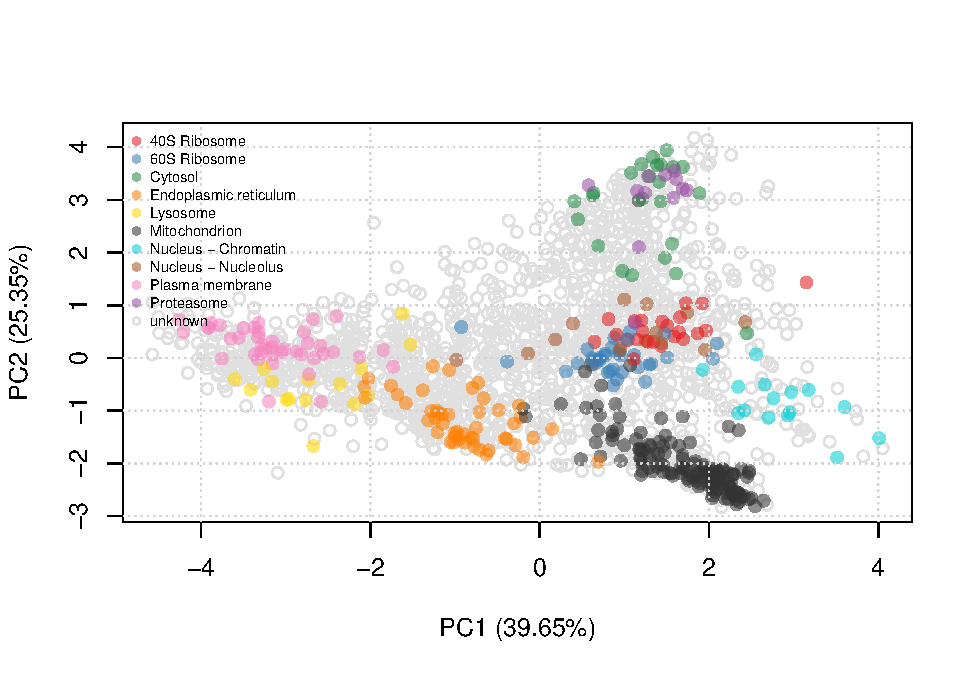
\includegraphics[width=0.7\linewidth]{F1000TAGMworkflow_files/figure-latex/e14pca1-1} 

}

\caption{First two principal components of mouse stem cell data.}\label{fig:e14pca1}
\end{figure}

\hypertarget{methods-tagm-map}{%
\section{\texorpdfstring{Methods: \emph{TAGM MAP}}{Methods: TAGM MAP}}\label{methods-tagm-map}}

\hypertarget{introduction-to-tagm-map}{%
\subsection{Introduction to TAGM MAP}\label{introduction-to-tagm-map}}

We can use \emph{maximum a posteriori} (MAP) estimation to perform
Bayesian parameter estimation for our model. The \emph{maximum a posteriori} estimate
is the mode of the posterior distribution and can be used to
provide a point estimate summary of the posterior localisation
probabilities. In contrast to TAGM MCMC (see later), it does not provide samples from the posterior
distribution, however it allows for faster inference by using an extended version of the
expectation-maximisation (EM) algorithm. The EM algorithm
iterates between an expectation step and a maximisation step. This
allows us to find parameters which maximise the logarithm of the
posterior, in the presence of latent (unobserved) variables. The EM
algorithm is guaranteed to converge to a local mode. The code chunk
below executes the \texttt{tagmMapTrain} function for a default of 100
iterations. We use the default priors for simplicity and convenience,
however they can be changed, which we explain in a later section. The
output is an object of class \texttt{MAPParams}, that captures the details of
the TAGM MAP model.

\begin{Shaded}
\begin{Highlighting}[]
\KeywordTok{set.seed}\NormalTok{(}\DecValTok{2}\NormalTok{)}
\NormalTok{mappars <-}\StringTok{ }\KeywordTok{tagmMapTrain}\NormalTok{(E14TG2aR)}
\end{Highlighting}
\end{Shaded}

\begin{verbatim}
## co-linearity detected; a small multiple of
##               the identity was added to the covariance
\end{verbatim}

\begin{Shaded}
\begin{Highlighting}[]
\NormalTok{mappars}
\end{Highlighting}
\end{Shaded}

\begin{verbatim}
## Object of class "MAPParams"
##  Method: MAP
\end{verbatim}

\hypertarget{aside-collinearity}{%
\subsubsection*{Aside: collinearity}\label{aside-collinearity}}
\addcontentsline{toc}{subsubsection}{Aside: collinearity}

The previous code chunk outputs a message concerning data collinearity.
This is because the covariance matrix of the data has become ill-conditioned
and as a result the inversion of this matrix becomes unstable with floating
point arithmetic. This can lead to the failure of standard matrix algorithms upon
which our method depends. In this case, it is standard practice to add a small
multiple of the identity to stabilise this matrix.
The printed message is a statement that this operation has been performed
for these data.

\hypertarget{model-visualisation}{%
\subsection{Model visualisation}\label{model-visualisation}}

The results of the modelling can be visualised with the \texttt{plotEllipse}
function on figure \ref{fig:e14ellipse}. The outer ellipse contains
99\% of the total probability whilst the middle and inner ellipses
contain 95\% and 90\% of the probability respectively. The centres of
the clusters are represented by black circumpunct (circled dot). We
can also plot the model in other principal components. The code chunk
below plots the probability ellipses along the first and second, as
well as the fourth principal component. The user can change the
components visualised by altering the \texttt{dims} argument.

\begin{Shaded}
\begin{Highlighting}[]
\KeywordTok{par}\NormalTok{(}\DataTypeTok{mfrow =} \KeywordTok{c}\NormalTok{(}\DecValTok{1}\NormalTok{, }\DecValTok{2}\NormalTok{))}
\KeywordTok{plotEllipse}\NormalTok{(E14TG2aR, mappars)}
\KeywordTok{plotEllipse}\NormalTok{(E14TG2aR, mappars, }\DataTypeTok{dims =} \KeywordTok{c}\NormalTok{(}\DecValTok{1}\NormalTok{, }\DecValTok{4}\NormalTok{))}
\end{Highlighting}
\end{Shaded}

\begin{figure}

{\centering 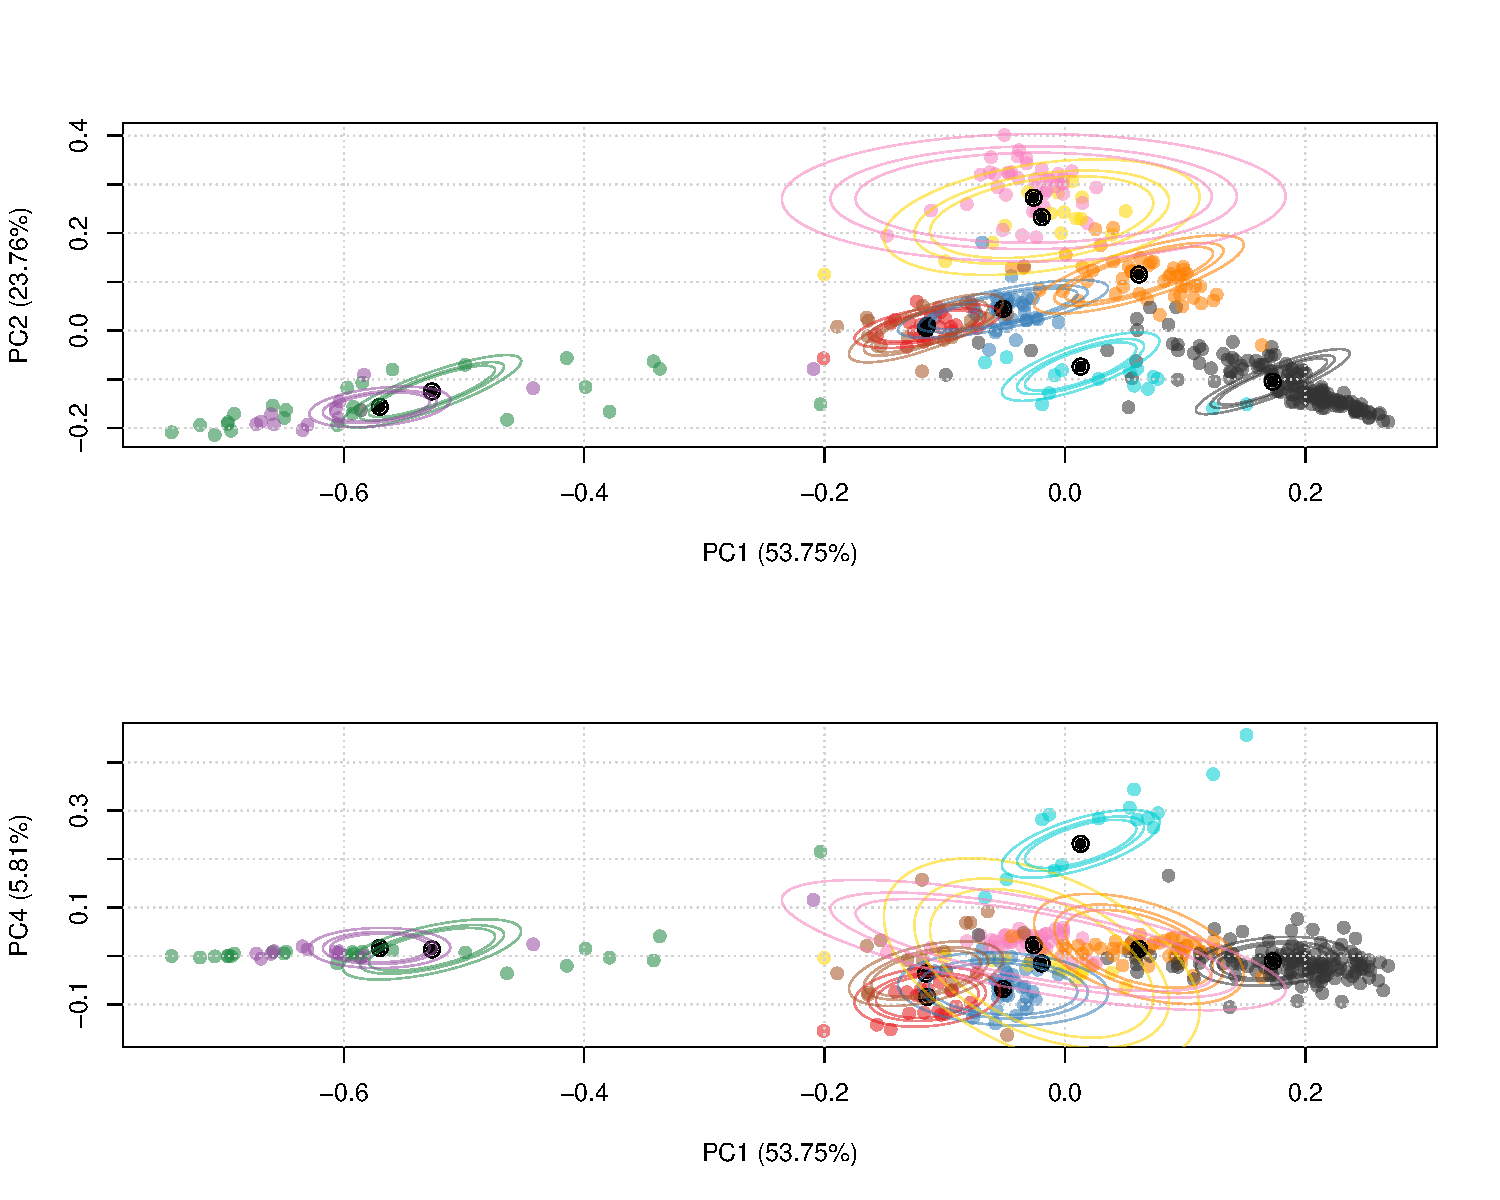
\includegraphics[width=1\linewidth]{F1000TAGMworkflow_files/figure-latex/e14ellipse-1} 

}

\caption{PCA plot with probability ellipses along PC 1 and 2 (left) and PC 1 and 4 (right).}\label{fig:e14ellipse}
\end{figure}

\hypertarget{the-expectation-maximisation-algorithm}{%
\subsection{The expectation-maximisation algorithm}\label{the-expectation-maximisation-algorithm}}

The EM algorithm is iterative; that is, the algorithm iterates between
an expectation step and a maximisation step until the value of the
log-posterior does not change \citep{EM:1977}. This fact can be used to
assess the convergence of the EM algorithm. The value of the
log-posterior at each iteration can be accessed with the
\texttt{logPosteriors} function on the \texttt{MAPParams} object. The code chuck
below plots the log posterior at each iteration and we see on figure
\ref{fig:mapconverge} the algorithm rapidly plateaus and so we have
achieved convergence. If convergence has not been reached during this
time, we suggest to increase the number of iterations by changing the
parameter \texttt{numIter} in the \texttt{tagmMapTrain} method. In practice, it is not
unexpected to observe small fluctuations due to numerical errors and
this should not concern users.

\begin{Shaded}
\begin{Highlighting}[]
\KeywordTok{plot}\NormalTok{(}\KeywordTok{logPosteriors}\NormalTok{(mappars), }\DataTypeTok{type =} \StringTok{"b"}\NormalTok{, }\DataTypeTok{col =} \StringTok{"blue"}\NormalTok{,}
     \DataTypeTok{cex =} \FloatTok{0.3}\NormalTok{, }\DataTypeTok{ylab =} \StringTok{"log-posterior"}\NormalTok{, }\DataTypeTok{xlab =} \StringTok{"iteration"}\NormalTok{)}
\end{Highlighting}
\end{Shaded}

\begin{figure}

{\centering 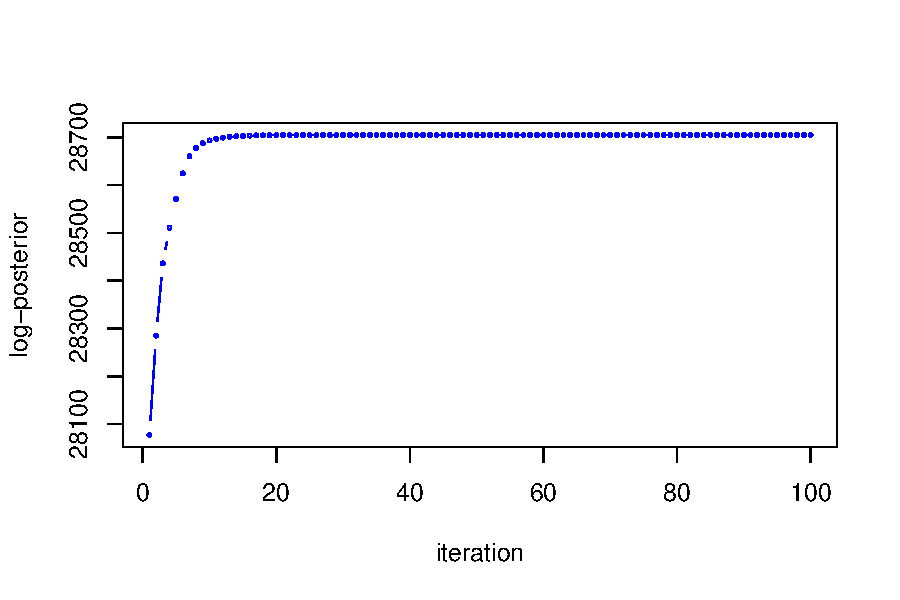
\includegraphics[width=0.8\linewidth]{F1000TAGMworkflow_files/figure-latex/mapconverge-1} 

}

\caption{Log-posterior at each iteration of the EM algorithm demonstrating convergence.}\label{fig:mapconverge}
\end{figure}

The code chuck below uses the \texttt{mappars} object generated above, along
with the \texttt{E14RG2aR} dataset, to classify the proteins of unknown localisation
using \texttt{tagmPredict} function. The results of running \texttt{tagmPredict} are
appended to the \texttt{fData} columns of the \texttt{MSnSet}.

\begin{Shaded}
\begin{Highlighting}[]
\NormalTok{E14TG2aR <-}\StringTok{ }\KeywordTok{tagmPredict}\NormalTok{(E14TG2aR, mappars) }\CommentTok{# Predict protein localisation}
\end{Highlighting}
\end{Shaded}

The new feature variables that are generated are:

\begin{itemize}
\item
  \texttt{tagm.map.allocation}: the TAGM MAP predictions for the most
  probable protein sub-cellular allocation.
\end{itemize}

\begin{Shaded}
\begin{Highlighting}[]
\KeywordTok{table}\NormalTok{(}\KeywordTok{fData}\NormalTok{(E14TG2aR)}\OperatorTok{$}\NormalTok{tagm.map.allocation)}
\end{Highlighting}
\end{Shaded}

\begin{verbatim}
## 
##          40S Ribosome          60S Ribosome               Cytosol 
##                    34                    85                   328 
## Endoplasmic reticulum              Lysosome         Mitochondrion 
##                   284                   147                   341 
##   Nucleus - Chromatin   Nucleus - Nucleolus       Plasma membrane 
##                   143                   322                   326 
##            Proteasome 
##                    21
\end{verbatim}

\begin{itemize}
\item
  \texttt{tagm.map.probability}: the posterior probability for the protein
  sub-cellular allocations.
\end{itemize}

\begin{Shaded}
\begin{Highlighting}[]
\KeywordTok{summary}\NormalTok{(}\KeywordTok{fData}\NormalTok{(E14TG2aR)}\OperatorTok{$}\NormalTok{tagm.map.probability)}
\end{Highlighting}
\end{Shaded}

\begin{verbatim}
##    Min. 1st Qu.  Median    Mean 3rd Qu.    Max. 
## 0.00000 0.06963 0.93943 0.63829 0.99934 1.00000
\end{verbatim}

\begin{itemize}
\item
  \texttt{tagm.map.outlier}: the posterior probability for that protein to
  belong to the outlier component rather than any annotated component.
\end{itemize}

\begin{Shaded}
\begin{Highlighting}[]
\KeywordTok{summary}\NormalTok{(}\KeywordTok{fData}\NormalTok{(E14TG2aR)}\OperatorTok{$}\NormalTok{tagm.map.outlier)}
\end{Highlighting}
\end{Shaded}

\begin{verbatim}
##      Min.   1st Qu.    Median      Mean   3rd Qu.      Max. 
## 0.0000000 0.0002363 0.0305487 0.3452624 0.9249810 1.0000000
\end{verbatim}

We can visualise the results by scaling the pointer according the
posterior localisation probabilities. To do this we extract the MAP
localisation probabilities from the feature columns of the the
\texttt{MSnSet} and pass these to the \texttt{plot2D} function (figure \ref{fig:mappca}).

\begin{Shaded}
\begin{Highlighting}[]
\NormalTok{ptsze <-}\StringTok{ }\KeywordTok{fData}\NormalTok{(E14TG2aR)}\OperatorTok{$}\NormalTok{tagm.map.probability }\CommentTok{# Scale pointer size}
\KeywordTok{plot2D}\NormalTok{(E14TG2aR, }\DataTypeTok{fcol =} \StringTok{"tagm.map.allocation"}\NormalTok{, }\DataTypeTok{cex =}\NormalTok{ ptsze)}
\KeywordTok{addLegend}\NormalTok{(E14TG2aR, }\DataTypeTok{where =} \StringTok{"topleft"}\NormalTok{, }\DataTypeTok{cex =} \FloatTok{0.6}\NormalTok{, }\DataTypeTok{fcol =} \StringTok{"tagm.map.allocation"}\NormalTok{)}
\end{Highlighting}
\end{Shaded}

\begin{figure}

{\centering 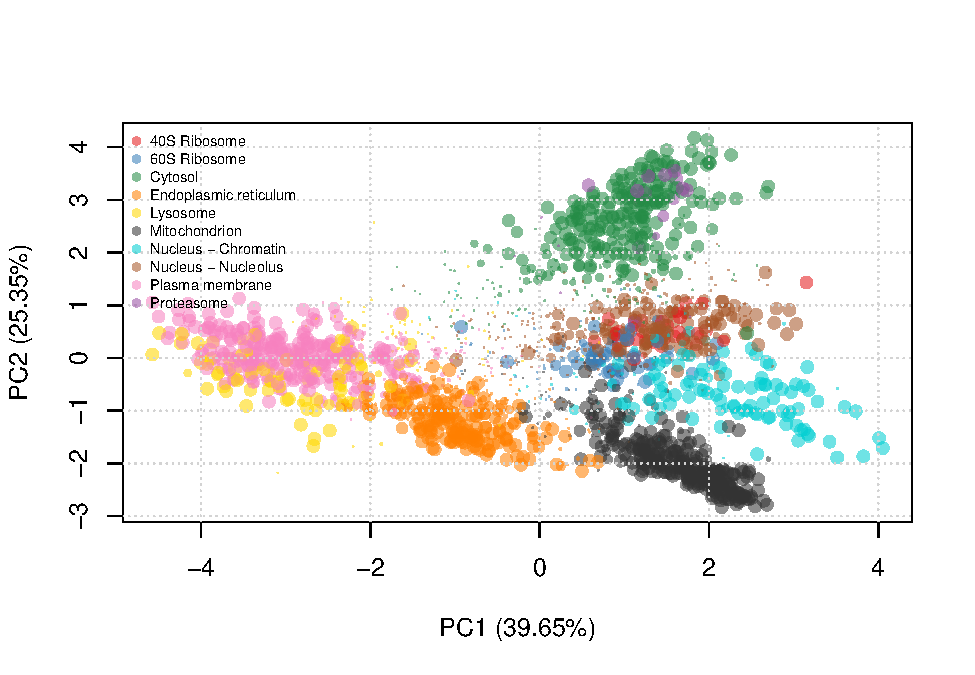
\includegraphics[width=0.7\linewidth]{F1000TAGMworkflow_files/figure-latex/mappca-1} 

}

\caption{TAGM MAP allocations, where the pointer is scaled according to the localisation probability and coloured according to the most probable subcellular niche.}\label{fig:mappca}
\end{figure}

The TAGM MAP method is easy to use and it is simple to check
convergence, however it is limited in that it can only provide point
estimates of the posterior localisation distributions. To obtain the
full posterior distributions and therefore a rich analysis of the
data, we use Markov-Chain Monte-Carlo methods. In our
particular case, we use a \emph{collapsed Gibbs sampler}
\citep{Smith:1993}.

\hypertarget{methods-tagm-mcmc-a-brief-overview}{%
\section{\texorpdfstring{Methods: \emph{TAGM MCMC} a brief overview}{Methods: TAGM MCMC a brief overview}}\label{methods-tagm-mcmc-a-brief-overview}}

The TAGM MCMC method allows a fully Bayesian analysis of spatial
proteomics datasets. It employs a collapsed Gibbs sampler to
sample from the posterior distribution of localisation probablities,
providing a rich analysis of the data. This section demonstrates the
advantage of taking a Bayesian approach and the biological information
that can be extracted from this analysis.

For those unfamiliar with Bayesian methodology,
some of the key ideas for a more complete
understanding are as follows. Firstly, MCMC based inference contrasts with MAP based
inference in that it \textit{samples} from the posterior
distribution of localisation probabilities. Hence, we do not just have
a single estimate for each quantity but a distribution of
estimates. MCMC methods are a large class of algorithms used to sample
from a probability distribution, in our case the posterior
distribution of the parameters \citep{Gilks:1995}. Once we have sampled from the posterior
distribution, we can estimate the mean of the posterior
distribution by simply taking the mean of the samples. In a similar
fashion, we can obtain estimates of other summaries of the posterior distribution.

A schematic of MCMC sampling is provided in figure
\ref{fig:mcmcCartoon} to aid understanding. Proteins, coloured blue,
are visualised along two variables of the data. Probability ellipses
representing contours of a probability distribution matching the
distribution of the proteins are overlaid. We now wish to obtain
samples from this distribution. The MCMC algorithm is initialised with
a starting location, then at each iteration a new value is
proposed. These proposed values are either accepted or rejected
(according to a carefully computed acceptance probability) and over
many iterations the algorithm converges and produces
samples from the desired distribution. Samples from the mean of this distribution
are coloured in red in the schematic figure. A large portion of the earlier
samples may not reflect the true distribution, because the MCMC
sampler has yet to converge. These early samples are usually discarded
and this is referred to as burn-in. The next state of the
algorithm depends on its current state and this leads to
auto-correlation in the samples. To suppress this auto-correlation, we
only retain every \(r^{th}\) sample. This is known as thinning. The details of burn-in and
thinning are further explained in later sections.

\begin{figure}

{\centering 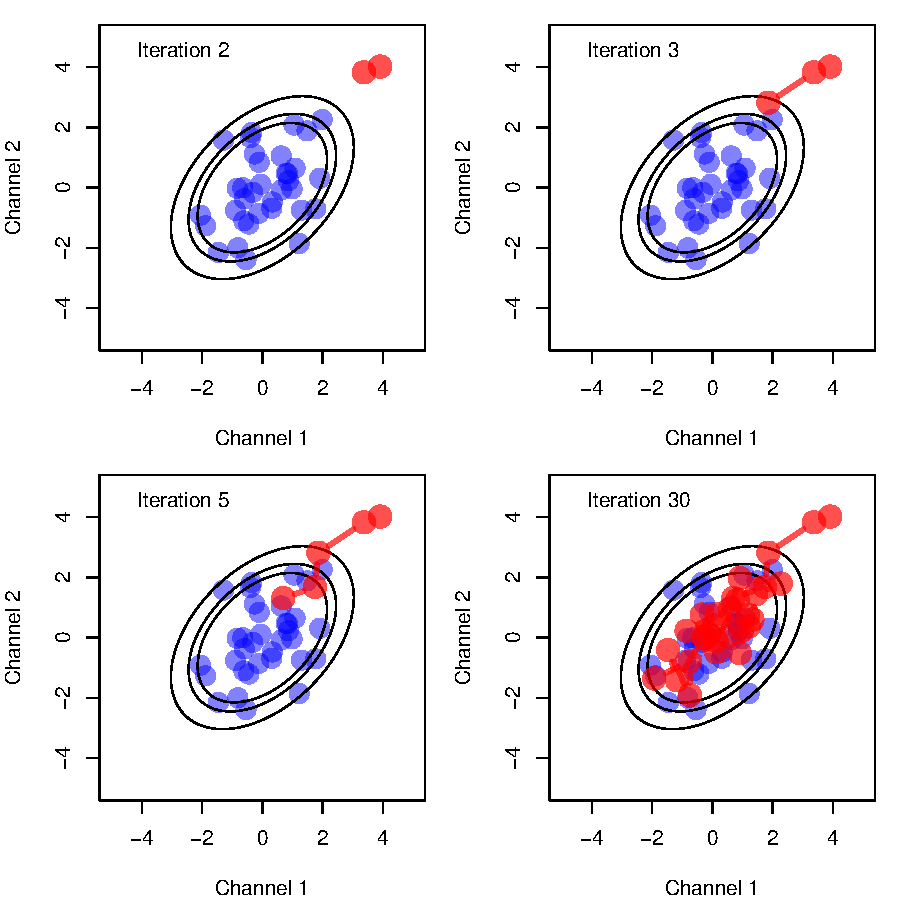
\includegraphics{F1000TAGMworkflow_files/figure-latex/mcmcCartoon-1} 

}

\caption{A schematic figure of MCMC sampling. Proteins are coloured in blue and probability ellipses are overlaid representing contours of a probability distribution matching the distribution of the proteins. MCMC samples from the mean of this distribution are then coloured in red.}\label{fig:mcmcCartoon}
\end{figure}

The TAGM MCMC method is computationally intensive and requires at
least modest processing power. Leaving the MCMC algorithm to run
overnight on a modern desktop is usually sufficient, however this, of
course, depends on the particular dataset being analysed. For guidance: it should not be expected that the
analysis will finish in just a couple of hours on a medium specification
laptop, for example.

To demonstrate the class structure and expected outputs of the TAGM
MCMC method, we run a brief analysis on a subset (400 randomly
chosen proteins) of the \texttt{tan2009r1} dataset from the \texttt{pRolocdata},
purely for illustration. This is to provide a bare bones analysis of
these data without being held back by computational requirements. We
perform a complete demonstration and provide precise details of the
analysis of the stem cell dataset considered above in the next
section.

\begin{Shaded}
\begin{Highlighting}[]
\KeywordTok{set.seed}\NormalTok{(}\DecValTok{1}\NormalTok{)}
\KeywordTok{data}\NormalTok{(tan2009r1)}
\NormalTok{tan2009r1 <-}\StringTok{ }\NormalTok{tan2009r1[}\KeywordTok{sample}\NormalTok{(}\KeywordTok{nrow}\NormalTok{(tan2009r1), }\DecValTok{400}\NormalTok{), ]}
\end{Highlighting}
\end{Shaded}

The first step is to run a few MCMC chains (below we use only 2 chains)
for a few iterations (we specify 3 iterations in the below code, but
typically we would suggest in the order of tens of thousands; see for
example the algorithms default settings by typing \texttt{?tagmMcmcTrain})
using the \texttt{tagmMcmcTrain} function. This function will generate a
object of class \texttt{MCMCParams}.

\begin{Shaded}
\begin{Highlighting}[]
\NormalTok{p <-}\StringTok{ }\KeywordTok{tagmMcmcTrain}\NormalTok{(}\DataTypeTok{object =}\NormalTok{ tan2009r1, }\DataTypeTok{numIter =} \DecValTok{3}\NormalTok{,}
                   \DataTypeTok{burnin =} \DecValTok{1}\NormalTok{, }\DataTypeTok{thin =} \DecValTok{1}\NormalTok{, }\DataTypeTok{numChains =} \DecValTok{2}\NormalTok{)}
\NormalTok{p}
\end{Highlighting}
\end{Shaded}

\begin{verbatim}
## Object of class "MCMCParams"
## Method: TAGM.MCMC 
## Number of chains: 2
\end{verbatim}

Information for each MCMC chain is contained within the chains
slot. If needed, this information can be accessed manually. The
function \texttt{tagmMcmcProcess} processes the \texttt{MCMCParams} object and populates
the summary slot.

\begin{Shaded}
\begin{Highlighting}[]
\NormalTok{p <-}\StringTok{ }\KeywordTok{tagmMcmcProcess}\NormalTok{(p)}
\NormalTok{p}
\end{Highlighting}
\end{Shaded}

\begin{verbatim}
## Object of class "MCMCParams"
## Method: TAGM.MCMC 
## Number of chains: 2 
## Summary available
\end{verbatim}

The summary slot has now been populated to include basic summaries of
the MCMC chains, such as organelle allocations and localisation
probabilities. Protein information can be appended to the feature
columns of the \texttt{MSnSet} by using the \texttt{tagmPredict} function, which
extracts the required information from the summary slot of the
\texttt{MCMCParams} object.

\begin{Shaded}
\begin{Highlighting}[]
\NormalTok{res <-}\StringTok{ }\KeywordTok{tagmPredict}\NormalTok{(}\DataTypeTok{object =}\NormalTok{ tan2009r1, }\DataTypeTok{params =}\NormalTok{ p)}
\end{Highlighting}
\end{Shaded}

We can now access new variables:

\begin{itemize}
\item
  \texttt{tagm.mcmc.allocation}: the TAGM MCMC prediction for the most likely
  protein sub-cellular annotation.
\end{itemize}

\begin{Shaded}
\begin{Highlighting}[]
\KeywordTok{table}\NormalTok{(}\KeywordTok{fData}\NormalTok{(res)}\OperatorTok{$}\NormalTok{tagm.mcmc.allocation)}
\end{Highlighting}
\end{Shaded}

\begin{verbatim}
## 
##  Cytoskeleton            ER         Golgi      Lysosome mitochondrion 
##            12            97            25             9            40 
##       Nucleus    Peroxisome            PM    Proteasome  Ribosome 40S 
##            25             3           101            29            30 
##  Ribosome 60S 
##            29
\end{verbatim}

\begin{itemize}
\item
  \texttt{tagm.mcmc.probability}: the mean posterior probability for the protein
  sub-cellular allocations.
\end{itemize}

\begin{Shaded}
\begin{Highlighting}[]
\KeywordTok{summary}\NormalTok{(}\KeywordTok{fData}\NormalTok{(res)}\OperatorTok{$}\NormalTok{tagm.mcmc.probability)}
\end{Highlighting}
\end{Shaded}

\begin{verbatim}
##    Min. 1st Qu.  Median    Mean 3rd Qu.    Max. 
##  0.3887  0.8997  0.9901  0.9093  1.0000  1.0000
\end{verbatim}

We can also access other useful summaries of the MCMC methods:

\begin{itemize}
\item
  \texttt{tagm.mcmc.outlier} the posterior probability for the protein
  to belong to the outlier component.
\item
  \texttt{tagm.mcmc.probability.lowerquantile} and \texttt{tagm.mcmc.probability.upperquantile}
  are the lower and upper boundaries to the equi-tailed 95\% credible interval
  of \texttt{tagm.mcmc.probability}.
\item
  \texttt{tagm.mcmc.mean.shannon} a Monte-Carlo averaged Shannon entropy,
  which is a measure of uncertainty in the allocations.
\end{itemize}

\hypertarget{methods-tagm-mcmc-the-details}{%
\section{\texorpdfstring{Methods: \emph{TAGM MCMC} the details}{Methods: TAGM MCMC the details}}\label{methods-tagm-mcmc-the-details}}

This section explains how to manually manipulate the MCMC output of
the TAGM model. In the code chunk below, we load a pre-computed
TAGM MCMC model. The data file \texttt{e14tagm.rda} is available online\footnote{\url{https://drive.google.com/open?id=1zozntDhE6YZ-q8wjtQ-lxZ66EEszOGYi}}
and is not directly loaded into this package due to its size. The file
itself if around 500mb, which is too large to directly load into a package.

\begin{Shaded}
\begin{Highlighting}[]
\KeywordTok{load}\NormalTok{(}\StringTok{"e14Tagm.rda"}\NormalTok{)}
\end{Highlighting}
\end{Shaded}

The following code, which is not evaluated dynamically, was used to
produce the \texttt{tagmE14} \texttt{MCMCParams} object. We run the MCMC algorithm
for 20,000 iterations with 10,000 iterations discarded for burn-in. We
then thin the chain by 20. We ran 6 chains in parallel and so we
obtain 500 samples for each of the 6 chains, totalling 3,000
samples. The resulting file is assumed to be in our working directory.

\begin{Shaded}
\begin{Highlighting}[]
\NormalTok{e14Tagm <-}\StringTok{ }\KeywordTok{tagmMcmcTrain}\NormalTok{(E14TG2aR,}
                         \DataTypeTok{numIter =} \DecValTok{20000}\NormalTok{,}
                         \DataTypeTok{burnin =} \DecValTok{10000}\NormalTok{,}
                         \DataTypeTok{thin =} \DecValTok{20}\NormalTok{,}
                         \DataTypeTok{numChains =} \DecValTok{6}\NormalTok{)}
\end{Highlighting}
\end{Shaded}

Manually inspecting the object, we see that it is a \texttt{MCMCParams}
object with 6 chains.

\begin{Shaded}
\begin{Highlighting}[]
\NormalTok{e14Tagm}
\end{Highlighting}
\end{Shaded}

\begin{verbatim}
## Object of class "MCMCParams"
## Method: TAGM.MCMC 
## Number of chains: 6
\end{verbatim}

\hypertarget{data-exploration-and-convergence-diagnostics}{%
\subsection{Data exploration and convergence diagnostics}\label{data-exploration-and-convergence-diagnostics}}

Assessing whether or not an MCMC algorithm has converged is
challenging. Assessing and diagnosing convergence is an active area of
research and throughout the 1990s many approaches were proposed
\citep{Geweke:1992, Gelman:1992, Roberts:1994, Brooks:1998}. We provide a
more detailed exploration of this issue, but readers should bare in
mind that the methods provided below are diagnostics and cannot
guarantee convergence. We direct readers to several important works in
the literature discussing the assessment of convergence. Users that do
not assess convergence and base their downstream analysis on
unconverged chains are likely to obtain poor quality results.

We first assess convergence using a parallel chains approach. We find
producing multiple chains is benificial not only for computational
advantages but also for analysis of convergence of our chains.

\begin{Shaded}
\begin{Highlighting}[]
\CommentTok{## Get number of chains}
\NormalTok{nChains <-}\StringTok{ }\KeywordTok{length}\NormalTok{(e14Tagm)}
\NormalTok{nChains}
\end{Highlighting}
\end{Shaded}

\begin{verbatim}
## [1] 6
\end{verbatim}

The following code chunks set up a manual convergence diagnostic
check. We make use of objects and methods in the package
\emph{\href{https://CRAN.R-project.org/package=coda}{coda}} to perform this
analysis \citep{coda}. Our function below automatically coerces our
objects into \emph{\href{https://CRAN.R-project.org/package=coda}{coda}} for
ease of analysis. We first calculate the total number of outliers at
each iteration of each chain and, if the algorithm has converged, this
number should be the same (or very similar) across all 6 chains.

\begin{Shaded}
\begin{Highlighting}[]
\CommentTok{## Convergence diagnostic to see if we need to discard any}
\CommentTok{## iterations or entire chains: compute the number of outliers for}
\CommentTok{## each iteration for each chain}
\NormalTok{out <-}\StringTok{ }\KeywordTok{mcmc_get_outliers}\NormalTok{(e14Tagm)}
\end{Highlighting}
\end{Shaded}

We can observe this from the trace plots and histograms for each MCMC
chain (figure \ref{fig:mcmctraceHidden}). Unconverged chains should be
discarded from downstream analysis.

\begin{figure}

{\centering 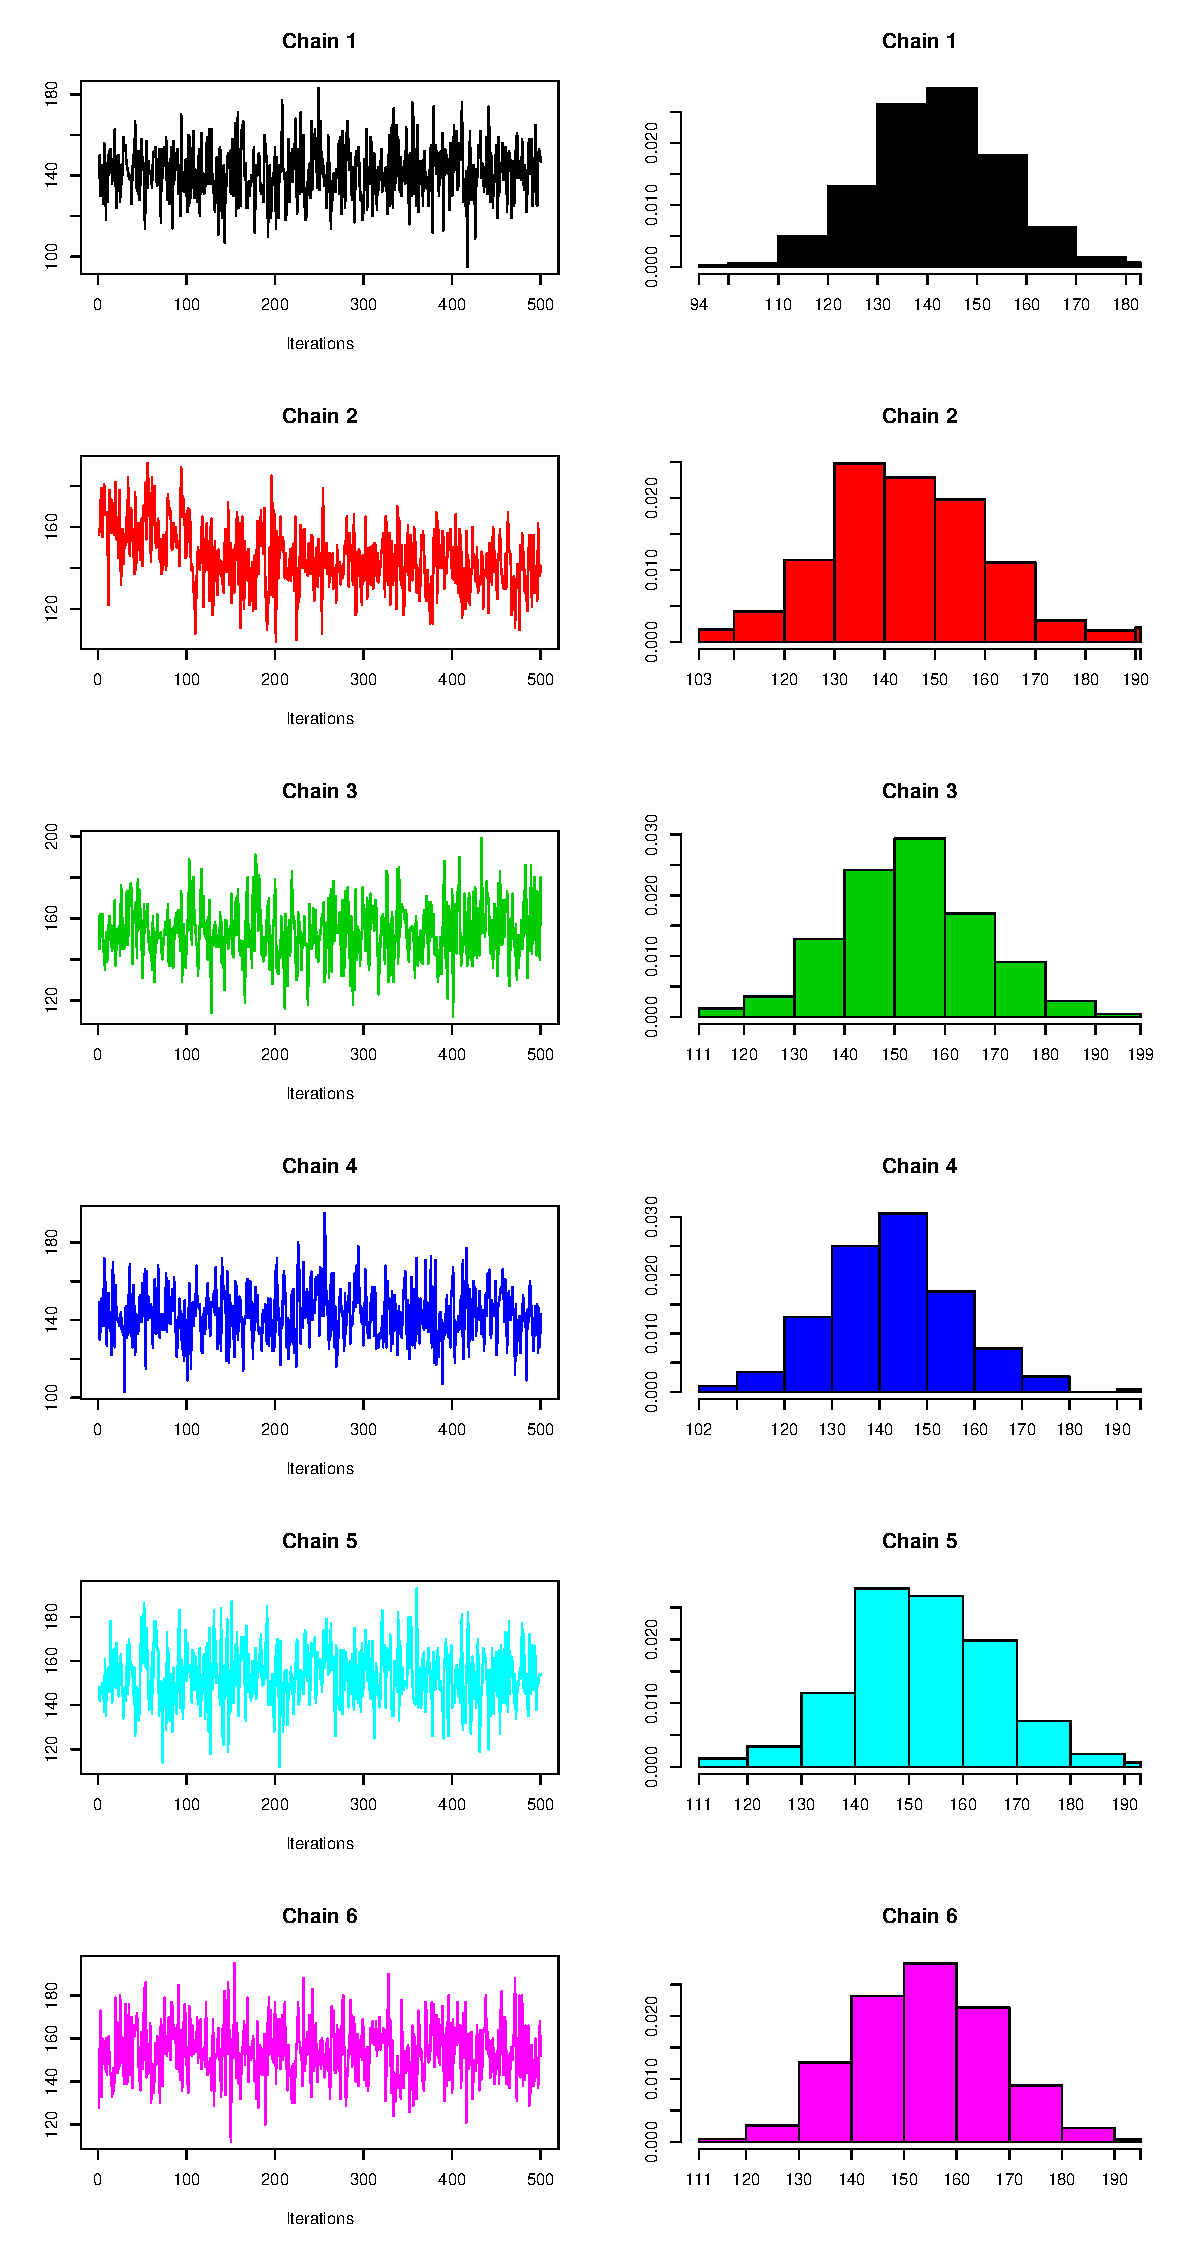
\includegraphics[width=0.7\linewidth]{F1000TAGMworkflow_files/figure-latex/mcmctraceHidden-1} 

}

\caption{Trace (left) and density (right) of the 6 MCMC chains.}\label{fig:mcmctraceHidden}
\end{figure}

\begin{Shaded}
\begin{Highlighting}[]
\CommentTok{## Using coda S3 objects to produce trace plots and histograms}
\ControlFlowTok{for}\NormalTok{ (i }\ControlFlowTok{in} \KeywordTok{seq_len}\NormalTok{(nChains))}
    \KeywordTok{plot}\NormalTok{(out[[i]], }\DataTypeTok{main =} \KeywordTok{paste}\NormalTok{(}\StringTok{"Chain"}\NormalTok{, i), }\DataTypeTok{auto.layout =} \OtherTok{FALSE}\NormalTok{, }\DataTypeTok{col =}\NormalTok{ i)}
\end{Highlighting}
\end{Shaded}

Chains 3, 5 and 6 are centred around an average of 153, with rapid
back and forth oscillations. Chain 2 should be immediately discarded,
since it has a large jump in the chain with clearly skewed
histogram. The other two chains oscillate differently with contrasting
quantiles to the 3 chains (3, 5 and 6) that agree with one another,
suggesting these chains have yet to converge. We can use the
\emph{\href{https://CRAN.R-project.org/package=coda}{coda}} package to produce
summaries of our chains. Here is the \texttt{coda} summary for the third
chain.

\begin{Shaded}
\begin{Highlighting}[]
\CommentTok{## Chains average around 153 outliers}
\KeywordTok{summary}\NormalTok{(out[[}\DecValTok{3}\NormalTok{]])}
\end{Highlighting}
\end{Shaded}

\begin{verbatim}
## 
## Iterations = 1:500
## Thinning interval = 1 
## Number of chains = 1 
## Sample size per chain = 500 
## 
## 1. Empirical mean and standard deviation for each variable,
##    plus standard error of the mean:
## 
##           Mean             SD       Naive SE Time-series SE 
##       153.4520        14.0771         0.6295         0.6820 
## 
## 2. Quantiles for each variable:
## 
##  2.5%   25%   50%   75% 97.5% 
##   127   144   153   162   183
\end{verbatim}

\hypertarget{applying-the-gelman-diagnostic}{%
\subsubsection{Applying the Gelman diagnostic}\label{applying-the-gelman-diagnostic}}

So far, our analysis appears promising. Three of our chains are centred around
an average of 153 outliers and there is no observed monotonicity in
our output. However, for a more rigorous and unbiased analysis of
convergence we can calculate the Gelman diagnostic using the
\emph{\href{https://CRAN.R-project.org/package=coda}{coda}} package
\citep{Gelman:1992, Brooks:1998}. This statistic is often referred to as
\(\hat{R}\) or the potential scale reduction factor. The idea of the
Gelman diagnostics is to compare the inter and intra chain
variances. The ratio of these quantities should be close to one. A more detailed and in depth discussion can be found
in the references. The \emph{\href{https://CRAN.R-project.org/package=coda}{coda}} package also
reports the \(95\%\) upper confidence interval of the \(\hat{R}\)
statistic. In this case, our samples are approximately normally distributed (see
histograms on the right in figure \ref{fig:mcmctraceHidden}). The
\emph{\href{https://CRAN.R-project.org/package=coda}{coda}} package allows for
transformations to improve normality of the data, and in some cases we
set the \texttt{transform} argument to apply log transformation. \citet{Gelman:1992}
suggest that chains with \(\hat{R}\) value of less than 1.2 are likely
to have converged.

\begin{Shaded}
\begin{Highlighting}[]
\KeywordTok{gelman.diag}\NormalTok{(out, }\DataTypeTok{transform =} \OtherTok{FALSE}\NormalTok{)}
\end{Highlighting}
\end{Shaded}

\begin{verbatim}
## Potential scale reduction factors:
## 
##      Point est. Upper C.I.
## [1,]       1.14       1.32
\end{verbatim}

\begin{Shaded}
\begin{Highlighting}[]
\KeywordTok{gelman.diag}\NormalTok{(out[}\KeywordTok{c}\NormalTok{(}\DecValTok{1}\NormalTok{,}\DecValTok{3}\NormalTok{,}\DecValTok{4}\NormalTok{,}\DecValTok{5}\NormalTok{,}\DecValTok{6}\NormalTok{)], }\DataTypeTok{transform =} \OtherTok{FALSE}\NormalTok{)}
\end{Highlighting}
\end{Shaded}

\begin{verbatim}
## Potential scale reduction factors:
## 
##      Point est. Upper C.I.
## [1,]       1.13       1.31
\end{verbatim}

\begin{Shaded}
\begin{Highlighting}[]
\KeywordTok{gelman.diag}\NormalTok{(out[}\KeywordTok{c}\NormalTok{(}\DecValTok{3}\NormalTok{,}\DecValTok{5}\NormalTok{,}\DecValTok{6}\NormalTok{)], }\DataTypeTok{transform =} \OtherTok{FALSE}\NormalTok{)}
\end{Highlighting}
\end{Shaded}

\begin{verbatim}
## Potential scale reduction factors:
## 
##      Point est. Upper C.I.
## [1,]          1       1.01
\end{verbatim}

In all cases, we see that the Gelman diagnostic for convergence is \textless{} 1.2.
However, the upper confidence interval is 1.32 when all chains are used; 1.31
when chain 2 is removed and when chains 1, 2 and 4 are removed the upper confidence interval
is 1.01 indicating that the MCMC algorithm for chains 3,5 and 6 might have converged.

We can also look at the Gelman diagnostics statistics for groups or
pairs of chains. The first line below computes the Gelman diagnostic
across the first three chains, whereas the second calculates the diagnostic
between chain 3 and chain 5.

\begin{Shaded}
\begin{Highlighting}[]
\KeywordTok{gelman.diag}\NormalTok{(out[}\DecValTok{1}\OperatorTok{:}\DecValTok{3}\NormalTok{], }\DataTypeTok{transform =} \OtherTok{FALSE}\NormalTok{) }\CommentTok{# the upper C.I is 1.62}
\end{Highlighting}
\end{Shaded}

\begin{verbatim}
## Potential scale reduction factors:
## 
##      Point est. Upper C.I.
## [1,]       1.22       1.62
\end{verbatim}

\begin{Shaded}
\begin{Highlighting}[]
\KeywordTok{gelman.diag}\NormalTok{(out[}\KeywordTok{c}\NormalTok{(}\DecValTok{3}\NormalTok{,}\DecValTok{5}\NormalTok{)], }\DataTypeTok{transform =} \OtherTok{TRUE}\NormalTok{) }\CommentTok{# the upper C.I is 1.01}
\end{Highlighting}
\end{Shaded}

\begin{verbatim}
## Potential scale reduction factors:
## 
##      Point est. Upper C.I.
## [1,]       1.01       1.01
\end{verbatim}

To assess another summary statistic, we can look at the mean
component allocation at each iteration of the MCMC algorithm and as
before we produce trace plots of this quantity (figure \ref{fig:mcmctrace2hidden}).

\begin{Shaded}
\begin{Highlighting}[]
\NormalTok{meanAlloc <-}\StringTok{ }\KeywordTok{mcmc_get_meanComponent}\NormalTok{(e14Tagm)}
\end{Highlighting}
\end{Shaded}

\begin{figure}

{\centering 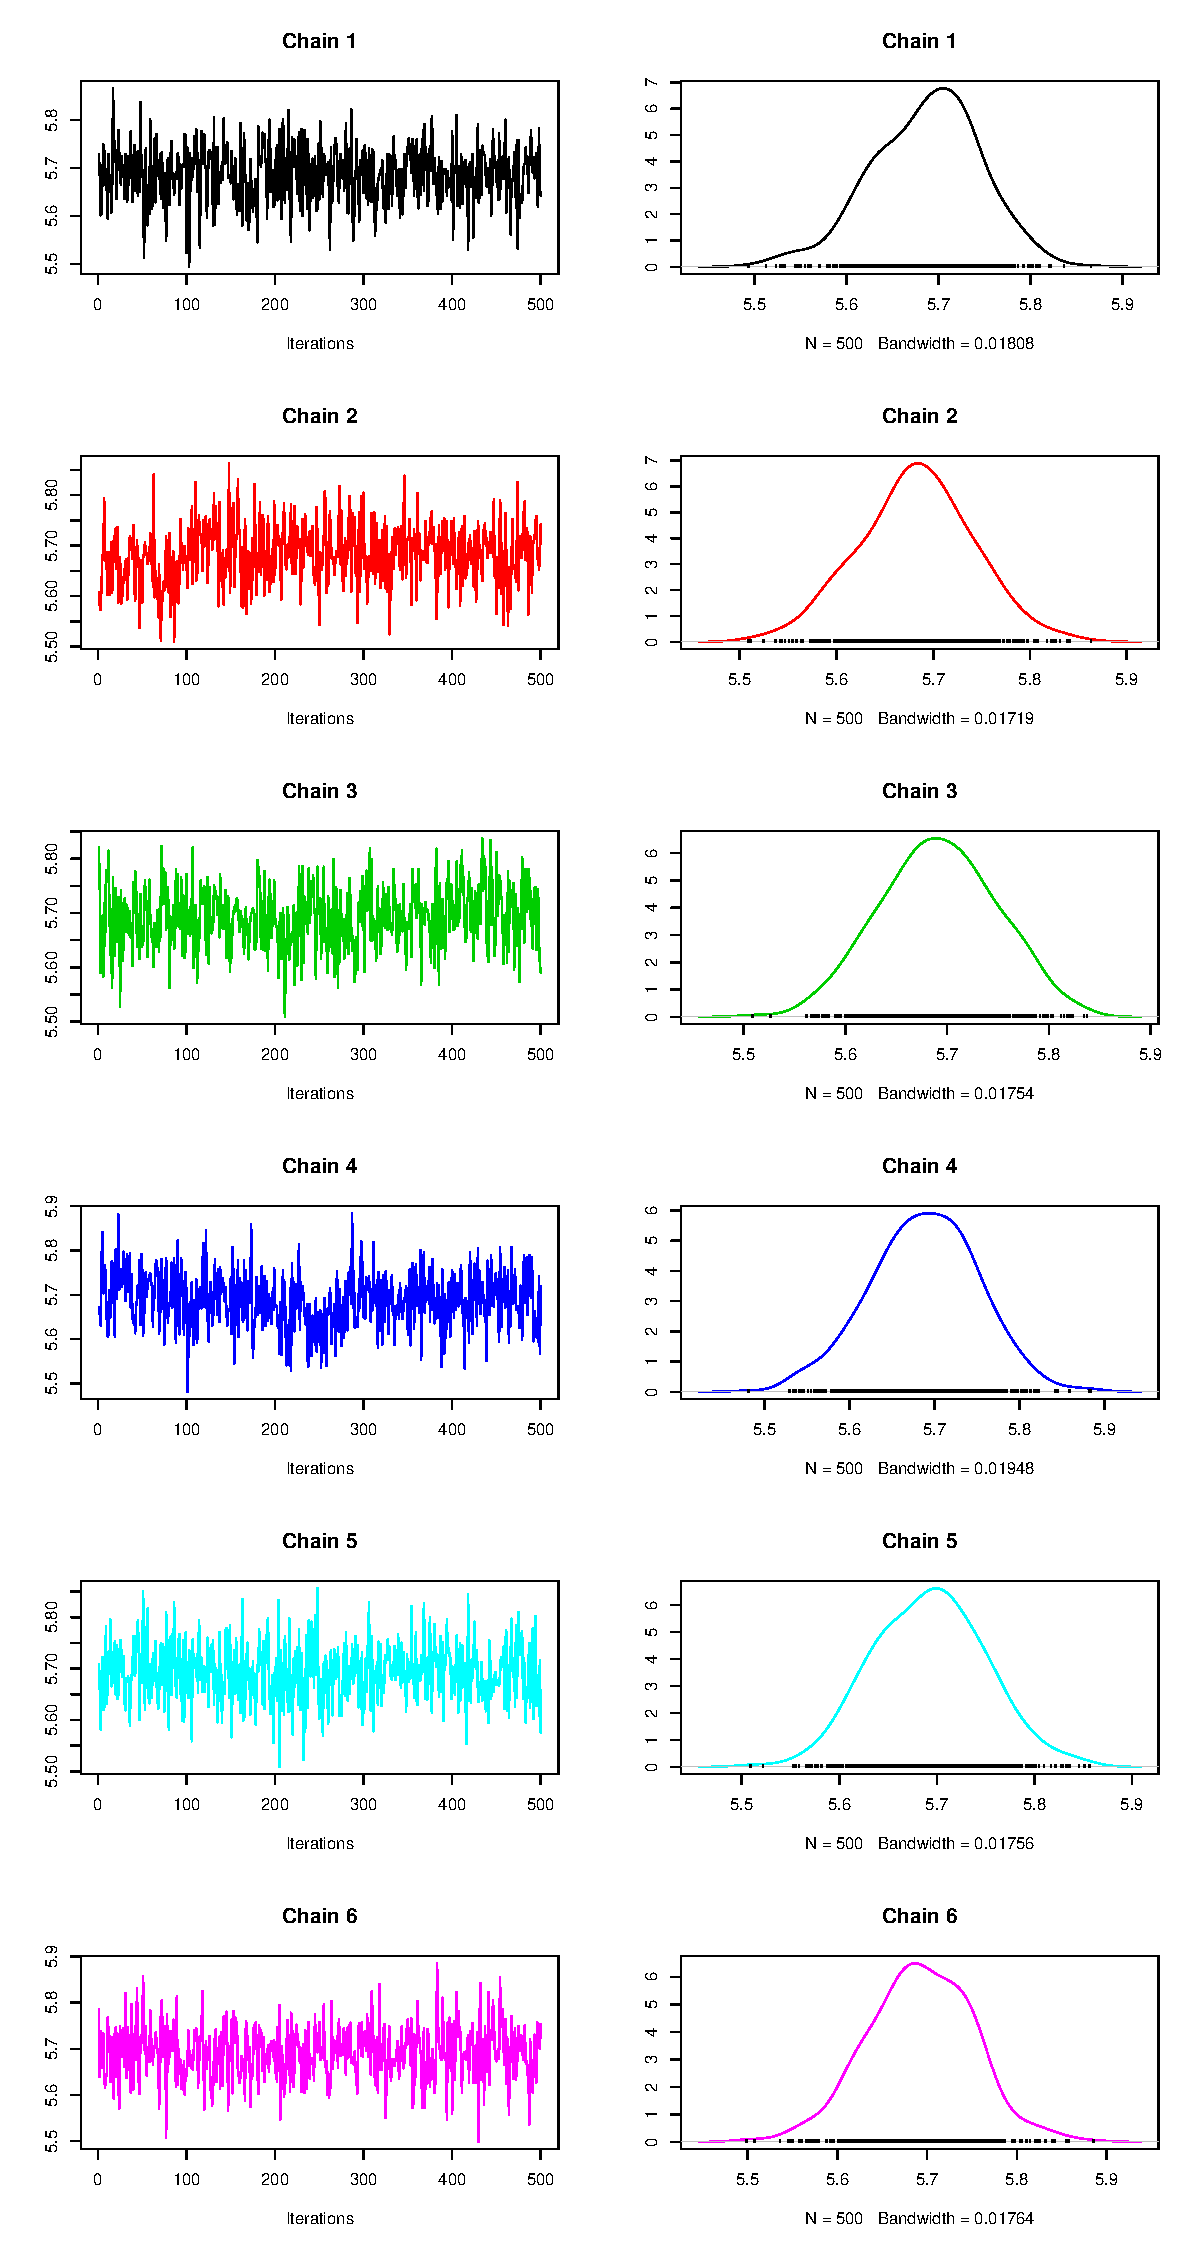
\includegraphics[width=0.7\linewidth]{F1000TAGMworkflow_files/figure-latex/mcmctrace2hidden-1} 

}

\caption{Trace (left) and density (right) of the mean component allocation of the 6 MCMC chains.}\label{fig:mcmctrace2hidden}
\end{figure}

\begin{Shaded}
\begin{Highlighting}[]
\ControlFlowTok{for}\NormalTok{ (i }\ControlFlowTok{in} \KeywordTok{seq_len}\NormalTok{(nChains))}
    \KeywordTok{plot}\NormalTok{(meanAlloc[[i]], }\DataTypeTok{main =} \KeywordTok{paste}\NormalTok{(}\StringTok{"Chain"}\NormalTok{, i), }\DataTypeTok{auto.layout =} \OtherTok{FALSE}\NormalTok{, }\DataTypeTok{col =}\NormalTok{ i)}
\end{Highlighting}
\end{Shaded}

As before we can produce summaries of the data.

\begin{Shaded}
\begin{Highlighting}[]
\KeywordTok{summary}\NormalTok{(meanAlloc[[}\DecValTok{1}\NormalTok{]])}
\end{Highlighting}
\end{Shaded}

\begin{verbatim}
## 
## Iterations = 1:500
## Thinning interval = 1 
## Number of chains = 1 
## Sample size per chain = 500 
## 
## 1. Empirical mean and standard deviation for each variable,
##    plus standard error of the mean:
## 
##           Mean             SD       Naive SE Time-series SE 
##       5.686713       0.059112       0.002644       0.002644 
## 
## 2. Quantiles for each variable:
## 
##  2.5%   25%   50%   75% 97.5% 
## 5.552 5.646 5.692 5.728 5.795
\end{verbatim}

We can already observe that there are some slight difference between
these chains which raises suspicion that some of the chains may not have converged.
For example each chain appears to be centred around 5.7, but chains 2 and 4
have clear jumps in the their trace plots. For a more quantitative
analysis, we again apply the Gelman diagnostics to these summaries.

\begin{Shaded}
\begin{Highlighting}[]
\KeywordTok{gelman.diag}\NormalTok{(meanAlloc)}
\end{Highlighting}
\end{Shaded}

\begin{verbatim}
## Potential scale reduction factors:
## 
##      Point est. Upper C.I.
## [1,]          1       1.01
\end{verbatim}

The above values are close to 1 and so we there are no significant difference
between the chains. As observed previously, chains 2 and 4
look quite different from the other chains and so we recalculate the diagnostic
excluding these chains. The computed Gelman diagnostic below suggest that chains 3, 5
and 6 have converged and that we should discard chains 1, 2 and 4 from
further analysis.

\begin{Shaded}
\begin{Highlighting}[]
\KeywordTok{gelman.diag}\NormalTok{(meanAlloc[}\KeywordTok{c}\NormalTok{(}\DecValTok{3}\NormalTok{,}\DecValTok{5}\NormalTok{,}\DecValTok{6}\NormalTok{)])}
\end{Highlighting}
\end{Shaded}

\begin{verbatim}
## Potential scale reduction factors:
## 
##      Point est. Upper C.I.
## [1,]          1          1
\end{verbatim}

For a further check, we can look at the mean outlier probability at
each iteration of the MCMC algorithm and again computing the Gelman
diagnostics between chains 4, 5 and 6. An \(\hat{R}\) statistics of
1 is indicative of convergence, since it is less than the recommend
value of 1.2.

\begin{Shaded}
\begin{Highlighting}[]
\NormalTok{meanoutProb <-}\StringTok{ }\KeywordTok{mcmc_get_meanoutliersProb}\NormalTok{(e14Tagm)}
\KeywordTok{gelman.diag}\NormalTok{(meanoutProb[}\KeywordTok{c}\NormalTok{(}\DecValTok{3}\NormalTok{, }\DecValTok{5}\NormalTok{, }\DecValTok{6}\NormalTok{)])}
\end{Highlighting}
\end{Shaded}

\begin{verbatim}
## Potential scale reduction factors:
## 
##      Point est. Upper C.I.
## [1,]          1       1.01
\end{verbatim}

\hypertarget{applying-the-geweke-diagnostic}{%
\subsubsection{Applying the Geweke diagnostic}\label{applying-the-geweke-diagnostic}}

Along with the Gelman diagnostic, which uses parallel chains, we can
also apply a single chain analysis using the Geweke diagnostic \citep{Geweke:1992}. The
Geweke diagnostic tests to see whether the mean calculated from the
first \(10\%\) of iterations is significantly different from the
mean calculated from the last \(50\%\) of iterations. If they are
significantly different, at say a level 0.01, then this is evidence
that particular chains have not converged. The following code chunk
calculates the Geweke diagnostic for each chain on the summarising
quantities we have previously computed.

\begin{Shaded}
\begin{Highlighting}[]
\KeywordTok{geweke_test}\NormalTok{(out)}
\end{Highlighting}
\end{Shaded}

\begin{verbatim}
##           chain 1      chain 2  chain 3    chain 4    chain 5    chain 6
## z.value 0.5749775 8.816632e+00 0.470203 -0.3204500 -0.6270787 -0.7328168
## p.value 0.5653065 1.179541e-18 0.638210  0.7486272  0.5306076  0.4636702
\end{verbatim}

\begin{Shaded}
\begin{Highlighting}[]
\KeywordTok{geweke_test}\NormalTok{(meanAlloc)}
\end{Highlighting}
\end{Shaded}

\begin{verbatim}
##           chain 1       chain 2    chain 3    chain 4   chain 5    chain 6
## z.value 1.1952967 -3.3737051063 -1.2232102 2.48951993 0.3605882 -0.1358850
## p.value 0.2319711  0.0007416377  0.2212503 0.01279157 0.7184073  0.8919122
\end{verbatim}

\begin{Shaded}
\begin{Highlighting}[]
\KeywordTok{geweke_test}\NormalTok{(meanoutProb)}
\end{Highlighting}
\end{Shaded}

\begin{verbatim}
##           chain 1      chain 2   chain 3    chain 4    chain 5     chain 6
## z.value 0.1785882 1.205500e+01 0.6189637 -0.5164987 -0.2141086 -0.02379004
## p.value 0.8582611 1.825379e-33 0.5359403  0.6055062  0.8304624  0.98102008
\end{verbatim}

The first test suggests chain 2 has not converged, since the p-value is
less than \(10^{-10}\) suggesting that the mean in the first \(10\%\) of
iterations is significantly different from those in the final
\(50\%\). Moreover, the second test and third tests also suggest that chain 2
has not converged. Furthermore, for the second test chain 4 has a marginally
small p-value, providing further evidence that this chain is of low quality. These
convergence diagnostics are not limited to the quantities we have
computed here and further diagnostics can be performed on any summary of
the data.

An important question to consider is whether removing an early portion
of the chain might lead to an improvement of the convergence diagnostics.
This might be particularly relevant if a chain converges some
iterations after our orginally specified \texttt{burn-in}. For example, let us
take the second Geweke test above, which suggested chains 2 and 4 had not
converged and see if discarding the initial \(10\%\) of the chain
improves the statistic. The function below removes \(50\) samples,
known as \texttt{burn-in}, from the beginning of each chain and the
output shows that we now have \(450\) samples in each chain. In practice,
as \(2\) chains are sufficient for good posterior estimates and convergence
we could simply discard chains \(2\) and \(4\) and proceed with downstream analysis
with the remaining chains.

\begin{Shaded}
\begin{Highlighting}[]
\NormalTok{burn_e14Tagm <-}\StringTok{ }\KeywordTok{mcmc_burn_chains}\NormalTok{(e14Tagm, }\DecValTok{50}\NormalTok{)}
\KeywordTok{chains}\NormalTok{(burn_e14Tagm)}
\end{Highlighting}
\end{Shaded}

\begin{verbatim}
## Object of class "MCMCChains"
##  Number of chains: 6
\end{verbatim}

\begin{Shaded}
\begin{Highlighting}[]
\KeywordTok{chains}\NormalTok{(burn_e14Tagm)[[}\DecValTok{4}\NormalTok{]]}
\end{Highlighting}
\end{Shaded}

\begin{verbatim}
## Object of class "MCMCChain"
##  Number of components: 10 
##  Number of proteins: 1663 
##  Number of iterations: 450
\end{verbatim}

The following function recomputes the number of outliers in each chain
at each iteration of each Markov-chain.

\begin{Shaded}
\begin{Highlighting}[]
\NormalTok{out2 <-}\StringTok{ }\KeywordTok{mcmc_get_outliers}\NormalTok{(burn_e14Tagm)}
\end{Highlighting}
\end{Shaded}

The code chuck below computes the Geweke diagnostic for this new
truncated chain and demonstrates that chain 4 has an improved Geweke
diagnostic, whilst chain 2 does not. Thus, in practice, it maybe
useful to remove iterations from the beginning of the chain. However,
as chain 4 did not pass the Gelman diagnostics we still discard it
from downstream analysis.

\begin{Shaded}
\begin{Highlighting}[]
\KeywordTok{geweke_test}\NormalTok{(out2)}
\end{Highlighting}
\end{Shaded}

\begin{verbatim}
##            chain 1      chain 2    chain 3   chain 4   chain 5   chain 6
## z.value -0.1455345 6.379618e+00 -1.6392215 0.3836940 0.1241201 0.6654703
## p.value  0.8842889 1.775298e-10  0.1011671 0.7012053 0.9012202 0.5057497
\end{verbatim}

\hypertarget{processing-converged-chains}{%
\subsection{Processing converged chains}\label{processing-converged-chains}}

Having made an assessment of convergence, we decide to discard chains
\(1,2\) and \(4\) from any further analysis. The code chunk below removes
these chains and creates a new object to store the converged chains.

\begin{Shaded}
\begin{Highlighting}[]
\NormalTok{removeChain <-}\StringTok{ }\KeywordTok{c}\NormalTok{(}\DecValTok{1}\NormalTok{, }\DecValTok{2}\NormalTok{, }\DecValTok{4}\NormalTok{) }\CommentTok{# The chains to be removed}
\NormalTok{e14Tagm_converged <-}\StringTok{ }\NormalTok{e14Tagm[}\OperatorTok{-}\NormalTok{removeChain] }\CommentTok{# Create new object}
\end{Highlighting}
\end{Shaded}

The \texttt{MCMCParams} object can be large and therefore if we have a large
number of samples we may want to subsample our chain, known
as \emph{thinning}, to reduce the number of samples. Thinning also has
another purpose. We may desire independent samples from our posterior
distribution but the MCMC algorithm produces auto-correlated
samples. Thinning can be applied to reduce the auto-correlation between
samples. The code chuck below, which is not evaluated, demonstrates
retaining every \(5^{th}\) iteration. Recall that we thinned by \(20\)
when we first ran the MCMC algorithm.

\begin{Shaded}
\begin{Highlighting}[]
\NormalTok{e14Tagm_converged_thinned <-}\StringTok{ }\KeywordTok{mcmc_thin_chains}\NormalTok{(e14Tagm_converged, }\DataTypeTok{freq  =} \DecValTok{5}\NormalTok{)}
\end{Highlighting}
\end{Shaded}

We initially ran \(6\) chains and, after having made an assessment of
convergence, we decided to discard \(3\) of the chains. We desire to make
inference using samples from all \(3\) chains, since this leads to better
posterior estimates. In their current class structure all the chains
are stored separately, so the following function pools all sample for
all chains together to make a single longer chain with all
samplers. Pooling a mixture of converged and unconverged chains is
likely to lead to poor quality results so should be done with care.

\begin{Shaded}
\begin{Highlighting}[]
\NormalTok{e14Tagm_converged_pooled <-}\StringTok{ }\KeywordTok{mcmc_pool_chains}\NormalTok{(e14Tagm_converged)}
\NormalTok{e14Tagm_converged_pooled}
\end{Highlighting}
\end{Shaded}

\begin{verbatim}
## Object of class "MCMCParams"
## Method: TAGM.MCMC 
## Number of chains: 1
\end{verbatim}

\begin{Shaded}
\begin{Highlighting}[]
\NormalTok{e14Tagm_converged_pooled[[}\DecValTok{1}\NormalTok{]]}
\end{Highlighting}
\end{Shaded}

\begin{verbatim}
## Object of class "MCMCChain"
##  Number of components: 10 
##  Number of proteins: 1663 
##  Number of iterations: 1500
\end{verbatim}

To populate the summary slot of the converged and pooled chain, we can use
the \texttt{tagmMcmcProcess} function. As we can see from the object below a summary
is now available. The information now available in the summary slot was detailed
in the previous section. We note that if there is more than \(1\) chain
in the \texttt{MCMCParams} object then the chains are automatically pooled
to compute the summaries.

\begin{Shaded}
\begin{Highlighting}[]
\NormalTok{e14Tagm_converged_pooled <-}\StringTok{ }\KeywordTok{tagmMcmcProcess}\NormalTok{(e14Tagm_converged_pooled)}
\NormalTok{e14Tagm_converged_pooled}
\end{Highlighting}
\end{Shaded}

\begin{verbatim}
## Object of class "MCMCParams"
## Method: TAGM.MCMC 
## Number of chains: 1 
## Summary available
\end{verbatim}

To create new feature columns in the \texttt{MSnSet} and append the summary
information, we apply the \texttt{tagmPredict} function. The \texttt{probJoint}
argument indicates whether or not to add probabilistic information for
all organelles for all proteins, rather than just the information for
the most probable organelle. The outlier probabilities are also returned
by default, but users can change this using the \texttt{probOutlier}
argument.

\begin{Shaded}
\begin{Highlighting}[]
\NormalTok{E14TG2aR <-}\StringTok{ }\KeywordTok{tagmPredict}\NormalTok{(}\DataTypeTok{object =}\NormalTok{ E14TG2aR,}
                        \DataTypeTok{params =}\NormalTok{ e14Tagm_converged_pooled,}
                        \DataTypeTok{probJoint =} \OtherTok{TRUE}\NormalTok{)}
\KeywordTok{head}\NormalTok{(}\KeywordTok{fData}\NormalTok{(E14TG2aR))}
\end{Highlighting}
\end{Shaded}

\begin{verbatim}
##        Uniprot.ID UniprotName
## Q62261     Q62261 SPTB2_MOUSE
## Q9JHU4     Q9JHU4 DYHC1_MOUSE
## Q9QXS1     Q9QXS1  PLEC_MOUSE
##                                     Protein.Description Peptides PSMs
## Q62261 Spectrin beta chain, brain 1 (multiple isoforms)       42   42
## Q9JHU4               Cytoplasmic dynein 1 heavy chain 1       33   33
## Q9QXS1                       Isoform PLEC-1I of Plectin       33   33
##        GOannotation markers.orig markers   tagm.map.allocation
## Q62261      PLM-SKE      unknown unknown Endoplasmic reticulum
## Q9JHU4          SKE      unknown unknown   Nucleus - Chromatin
## Q9QXS1      unknown      unknown unknown       Plasma membrane
##        tagm.map.probability tagm.map.outlier  tagm.mcmc.allocation
## Q62261         8.165817e-09     0.9999999857 Endoplasmic reticulum
## Q9JHU4         9.996798e-01     0.0003202255   Nucleus - Chromatin
## Q9QXS1         1.250898e-06     0.9999987491            Proteasome
##        tagm.mcmc.probability tagm.mcmc.probability.lowerquantile
## Q62261             0.5765793                        0.0020296117
## Q9JHU4             0.9738206                        0.7594516090
## Q9QXS1             0.4957129                        0.0002886457
##        tagm.mcmc.probability.upperquantile tagm.mcmc.mean.shannon
## Q62261                           0.9992504            0.201623229
## Q9JHU4                           0.9998822            0.081450206
## Q9QXS1                           0.9947100            0.447665536
##        tagm.mcmc.outlier tagm.mcmc.joint.40S Ribosome
## Q62261      2.547793e-01                 4.401228e-10
## Q9JHU4      3.335134e-05                 1.936225e-18
## Q9QXS1      6.423799e-01                 2.213861e-07
##        tagm.mcmc.joint.60S Ribosome tagm.mcmc.joint.Cytosol
## Q62261                 2.778620e-07            2.650861e-12
## Q9JHU4                 1.645727e-21            1.887645e-17
## Q9QXS1                 1.495170e-01            9.062280e-09
##        tagm.mcmc.joint.Endoplasmic reticulum tagm.mcmc.joint.Lysosome
## Q62261                          5.765793e-01             1.108757e-11
## Q9JHU4                          1.548053e-17             5.577415e-24
## Q9QXS1                          1.768681e-04             1.150706e-04
##        tagm.mcmc.joint.Mitochondrion tagm.mcmc.joint.Nucleus - Chromatin
## Q62261                  5.020528e-08                        4.231731e-01
## Q9JHU4                  2.835919e-22                        9.738206e-01
## Q9QXS1                  5.832273e-19                        7.920397e-03
##        tagm.mcmc.joint.Nucleus - Nucleolus tagm.mcmc.joint.Plasma membrane
## Q62261                        1.279255e-05                    1.914808e-11
## Q9JHU4                        2.617943e-02                    3.514851e-29
## Q9QXS1                        1.130580e-05                    3.465462e-01
##        tagm.mcmc.joint.Proteasome
## Q62261               2.345204e-04
## Q9JHU4               7.841425e-11
## Q9QXS1               4.957129e-01
##  [ reached getOption("max.print") -- omitted 2 rows ]
##  [ reached 'max' / getOption("max.print") -- omitted 1 rows ]
\end{verbatim}

\hypertarget{aside-priors}{%
\subsubsection*{\texorpdfstring{Aside: \emph{Priors}}{Aside: Priors}}\label{aside-priors}}
\addcontentsline{toc}{subsubsection}{Aside: \emph{Priors}}

Bayesian analysis requires users to specify prior information about
the parameters. This may appear to be a challenging task; however,
good default options are often possible. Should expert information be
available for any of these priors then the users should provide this,
otherwise we have found that the default choices work well in
practice. The priors also provide regularisation and shrinkage to
avoid overfitting. Given enough data the likelihood overwhelms the
prior and the influence of the prior is weak.

We place a normal inverse-Wishart prior on the parameters of the
mutivariate normal mixture components. The normal inverse-Wishart
prior has \(4\) hyperparameters that must be specified. These are: the
prior mean \texttt{mu0} expressing the prior location of each organelle; a
prior shrinkage \texttt{lambda0}, which is a scalar expressing uncertainty in
the prior mean; the prior degrees of freedom \texttt{nu0}; and a scale prior
\texttt{S0} on the covariance. Together, \texttt{nu0} and \texttt{S0} specify the prior
variability on organelle covariances. The same prior distribution is
assumed for the parameters of all mutivariate normal mixture
components.

The default options for these are based on the
choice recommended by \citep{Fraley:2005}. The prior mean \texttt{mu0} is set to
be the mean of the data. \texttt{lambda0} is set to be \(0.01\) meaning some
uncertainty in the covariance is propagated to the mean, increasing
\texttt{lambda0} increases shrinkage towards the prior. \texttt{nu0} is set to the
number of feature variables plus \(2\), which is the smallest integer
value that ensures a finite covariance matrix. The prior scale
matrix \(S0\) is set to

\begin{equation}
S_0 = \frac{\mathop{\mathrm{diag}}(\frac{1}{n}\sum (X - \bar{X})^2)}{K^{1/D}},
\end{equation}

and represents a diffuse prior on the covariance. Another good choice
which is often used is a constant multiple of the identity matrix. The
prior for the Dirichlet distribution concentration parameters \texttt{beta0}
is set to \(1\) for each organelle. Another
reasonable choice would be the non-informative Jeffery's prior for the
Dirichlet hyperparameter, which sets \texttt{beta0} to \(0.5\) for each
organelle. The prior weight for the outlier detection class is
a \(\mathcal{B}(u, v)\) distribution. The default for \(u = 2\) and the
default for \(v = 10\). This represents the reasonable belief that
\(\frac{u}{u + v} = \frac{1}{6}\)
proteins \emph{a priori} might be an outlier and we believe is unlikely that
more than \(50\%\) of proteins are outliers. Decreasing the value of \(v\),
represents more uncertainty about the number of protein that are
outliers.

\hypertarget{analysis-visualisation-and-interpretation-of-results}{%
\subsection{Analysis, visualisation and interpretation of results}\label{analysis-visualisation-and-interpretation-of-results}}

Now that we have a single pooled chain of samples from a converged MCMC
algorithm, we can begin to analyse the results. Preliminary analysis
includes visualising the allocated organelle and localisation
probability of each protein to its most probable organelle, as shown on
figure \ref{fig:mcmcpca}.

\begin{Shaded}
\begin{Highlighting}[]
\KeywordTok{par}\NormalTok{(}\DataTypeTok{mfrow =} \KeywordTok{c}\NormalTok{(}\DecValTok{1}\NormalTok{, }\DecValTok{2}\NormalTok{))}
\KeywordTok{plot2D}\NormalTok{(E14TG2aR, }\DataTypeTok{fcol =} \StringTok{"tagm.mcmc.allocation"}\NormalTok{,}
       \DataTypeTok{cex =} \KeywordTok{fData}\NormalTok{(E14TG2aR)}\OperatorTok{$}\NormalTok{tagm.mcmc.probability,}
       \DataTypeTok{main =} \StringTok{"TAGM MCMC allocations"}\NormalTok{)}
\KeywordTok{addLegend}\NormalTok{(E14TG2aR, }\DataTypeTok{fcol =} \StringTok{"markers"}\NormalTok{,}
          \DataTypeTok{where =} \StringTok{"topleft"}\NormalTok{, }\DataTypeTok{ncol =} \DecValTok{2}\NormalTok{, }\DataTypeTok{cex =} \FloatTok{0.6}\NormalTok{)}

\KeywordTok{plot2D}\NormalTok{(E14TG2aR, }\DataTypeTok{fcol =} \StringTok{"tagm.mcmc.allocation"}\NormalTok{,}
       \DataTypeTok{cex =} \KeywordTok{fData}\NormalTok{(E14TG2aR)}\OperatorTok{$}\NormalTok{tagm.mcmc.mean.shannon,}
       \DataTypeTok{main =} \StringTok{"Visualising global uncertainty"}\NormalTok{)}
\KeywordTok{addLegend}\NormalTok{(E14TG2aR, }\DataTypeTok{fcol =} \StringTok{"markers"}\NormalTok{,}
          \DataTypeTok{where =} \StringTok{"topleft"}\NormalTok{, }\DataTypeTok{ncol =} \DecValTok{2}\NormalTok{, }\DataTypeTok{cex =} \FloatTok{0.6}\NormalTok{)}
\end{Highlighting}
\end{Shaded}

\begin{figure}

{\centering 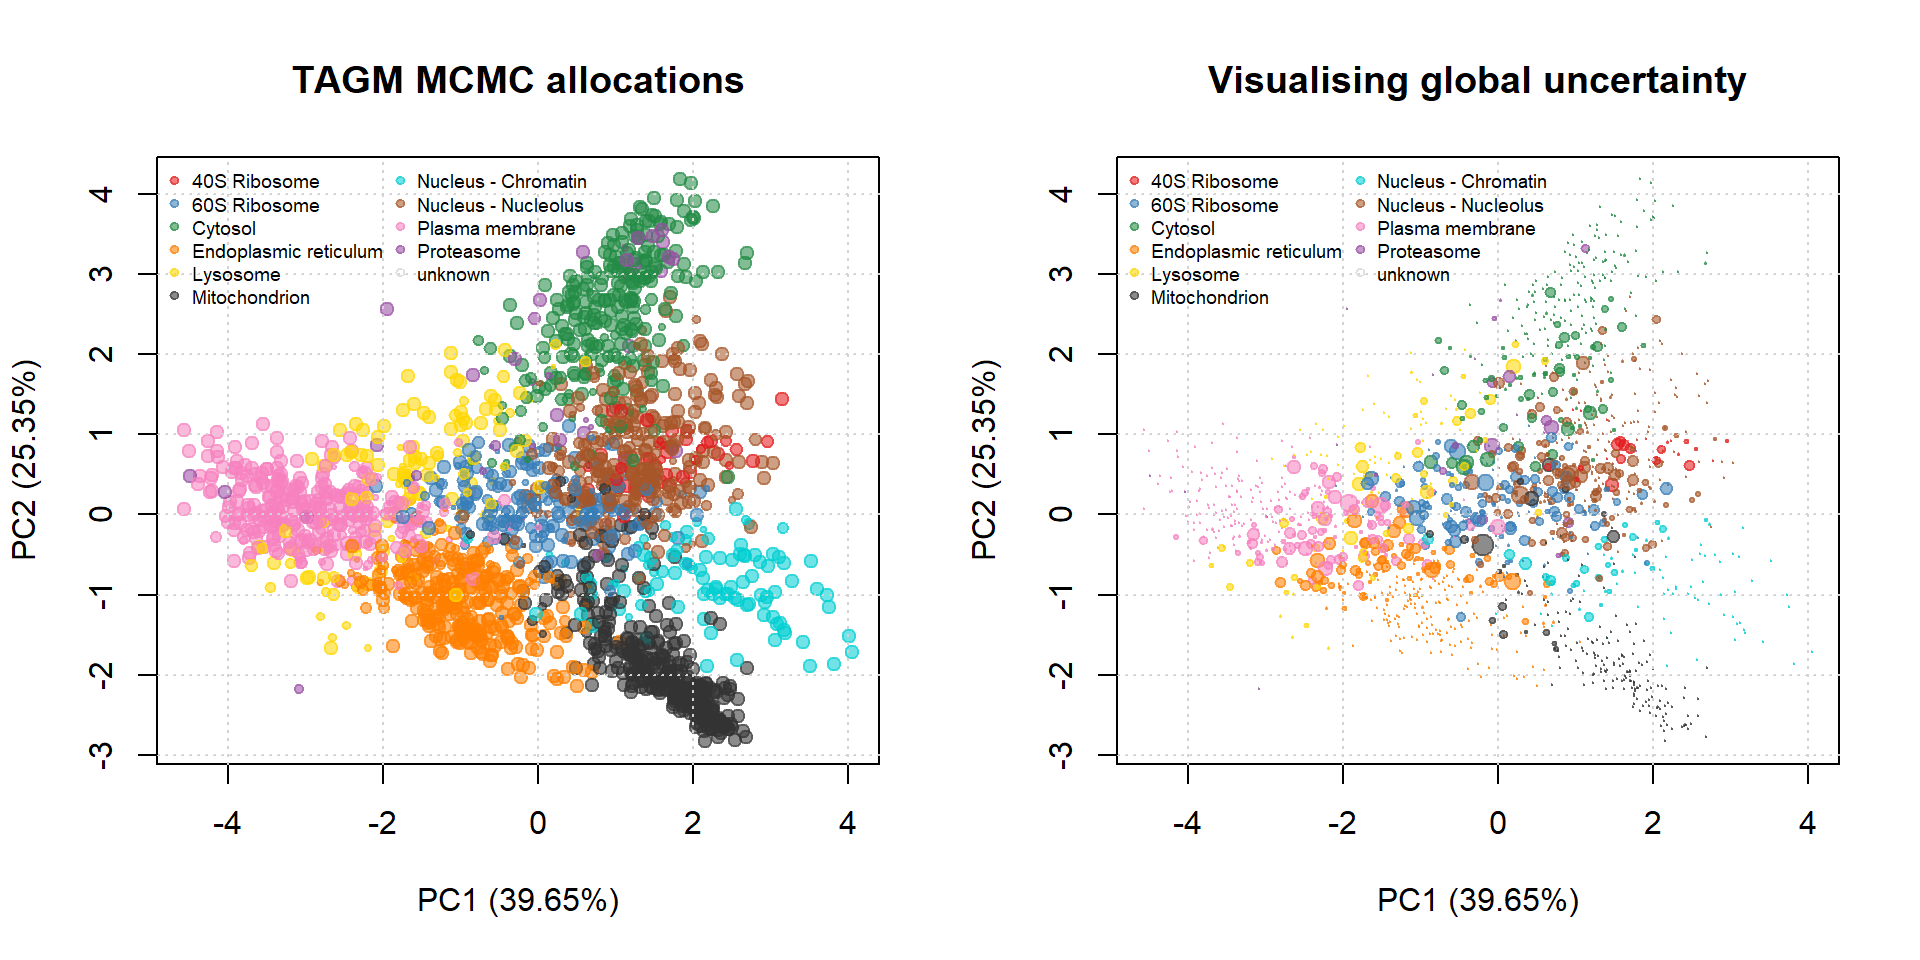
\includegraphics[width=1\linewidth]{F1000TAGMworkflow_files/figure-latex/mcmcpca-1} 

}

\caption{TAGM MCMC allocations. On the left, point size have been scaled based on allocation probabilities. On the right, the point size have been scaled based on the global uncertainty using the mean Shannon entropy.}\label{fig:mcmcpca}
\end{figure}

We can visualise other summaries of the data including a Monte-Carlo
averaged Shannon entropy, as shown in figure \ref{fig:mcmcpca} on the
right. This is a measure of uncertainty and proteins with greater
Shannon entropy have more uncertainty in their localisation. We
observe global patterns of uncertainty, particularly in areas where
organelle boundaries overlap. There are also regions of low
uncertainty indicating little doubt about the localisation of these
proteins.

We are also interested in the relationship between localisation
probability to the most probable class and the Shannon
entropy. Even though the two quantities are evidently correlated there
is still considerable spread. Thus it is important to base inference
not only on localisation probability but also a measure of uncertainty,
for example the Shannon entropy. Proteins with low Shannon entropy
have low uncertainty in their localisation, whilst those with higher Shannon
entropy have uncertain localisation. Since multi-localised protein have
uncertain localisation to a single subcellular niche, exploring the Shannon
can aid in identifying multi-localised proteins.

\begin{Shaded}
\begin{Highlighting}[]
\NormalTok{cls <-}\StringTok{ }\KeywordTok{getStockcol}\NormalTok{()[}\KeywordTok{as.factor}\NormalTok{(}\KeywordTok{fData}\NormalTok{(E14TG2aR)}\OperatorTok{$}\NormalTok{tagm.mcmc.allocation)]}
\KeywordTok{plot}\NormalTok{(}\KeywordTok{fData}\NormalTok{(E14TG2aR)}\OperatorTok{$}\NormalTok{tagm.mcmc.probability,}
     \KeywordTok{fData}\NormalTok{(E14TG2aR)}\OperatorTok{$}\NormalTok{tagm.mcmc.mean.shannon,}
     \DataTypeTok{col =}\NormalTok{ cls, }\DataTypeTok{pch =} \DecValTok{19}\NormalTok{,}
     \DataTypeTok{xlab =} \StringTok{"Localisation probability"}\NormalTok{,}
     \DataTypeTok{ylab =} \StringTok{"Shannon entropy"}\NormalTok{)}
\KeywordTok{addLegend}\NormalTok{(E14TG2aR, }\DataTypeTok{fcol =} \StringTok{"markers"}\NormalTok{,}
          \DataTypeTok{where =} \StringTok{"topright"}\NormalTok{, }\DataTypeTok{ncol =} \DecValTok{2}\NormalTok{, }\DataTypeTok{cex =} \FloatTok{0.6}\NormalTok{)}
\end{Highlighting}
\end{Shaded}

\begin{figure}

{\centering 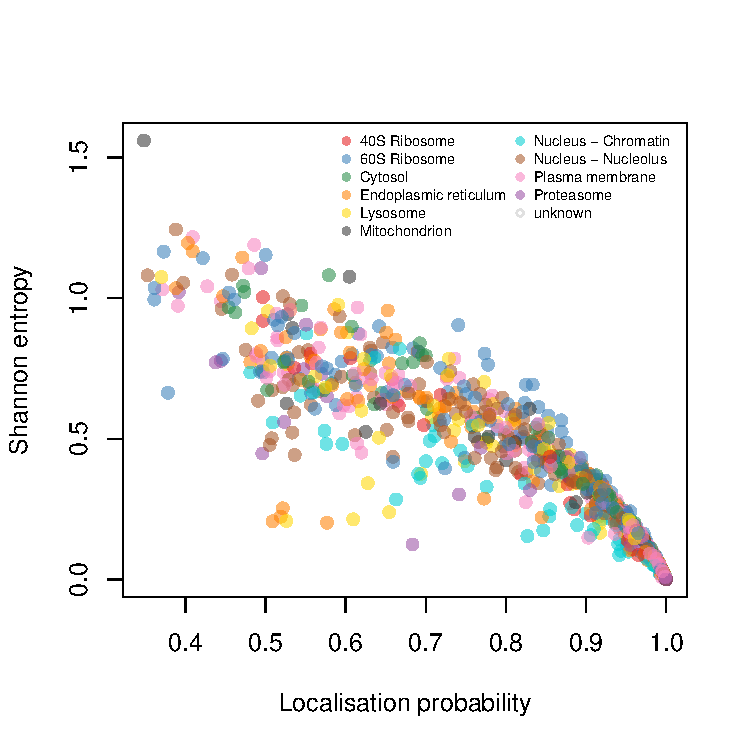
\includegraphics[width=0.7\linewidth]{F1000TAGMworkflow_files/figure-latex/probvsentr-1} 

}

\caption{Shannon entropy and localisation probability.}\label{fig:probvsentr}
\end{figure}

Aside from global visualisation of the data, we can also interrogate
each individual protein. As illustrated on figure
\ref{fig:probdists1}, we can obtain the full posterior distribution
of localisation probabilities for each protein from the
\texttt{e14Tagm\_converged\_pooled} object. We can use the \texttt{plot} generic on
the \texttt{MCMCParams} object to obtain a violin plot of the localisation
distribution. Simply providing the name of the protein in the second
argument produces the plot for that protein. The solute carrier
transporter protein E9QMX3, also referred to as Slc15a1, is most
probably localised to plasma membrane in line with its role as a
transmembrane transporter but also shows some uncertainty, potentially
also localising to other comparments. The first violin plot
visualises this uncertainty. The protein Q3V1Z5 is a supposed
constitute of the 40S ribosome and has poor UniProt annotation with
evidence only at the transcript level. From the plot below is is clear
that Q3V1Z5 is a ribosomal associated protein, but it previous
localisation has only been computational inferred and here we provide
experimental evidence of a ribosomal annotation. Thus, quantifying
uncertainty recovers important additional annotations.

\begin{Shaded}
\begin{Highlighting}[]
\KeywordTok{plot}\NormalTok{(e14Tagm_converged_pooled, }\StringTok{"E9QMX3"}\NormalTok{)}
\KeywordTok{plot}\NormalTok{(e14Tagm_converged_pooled, }\StringTok{"Q3V1Z5"}\NormalTok{)}
\end{Highlighting}
\end{Shaded}

\begin{figure}

{\centering 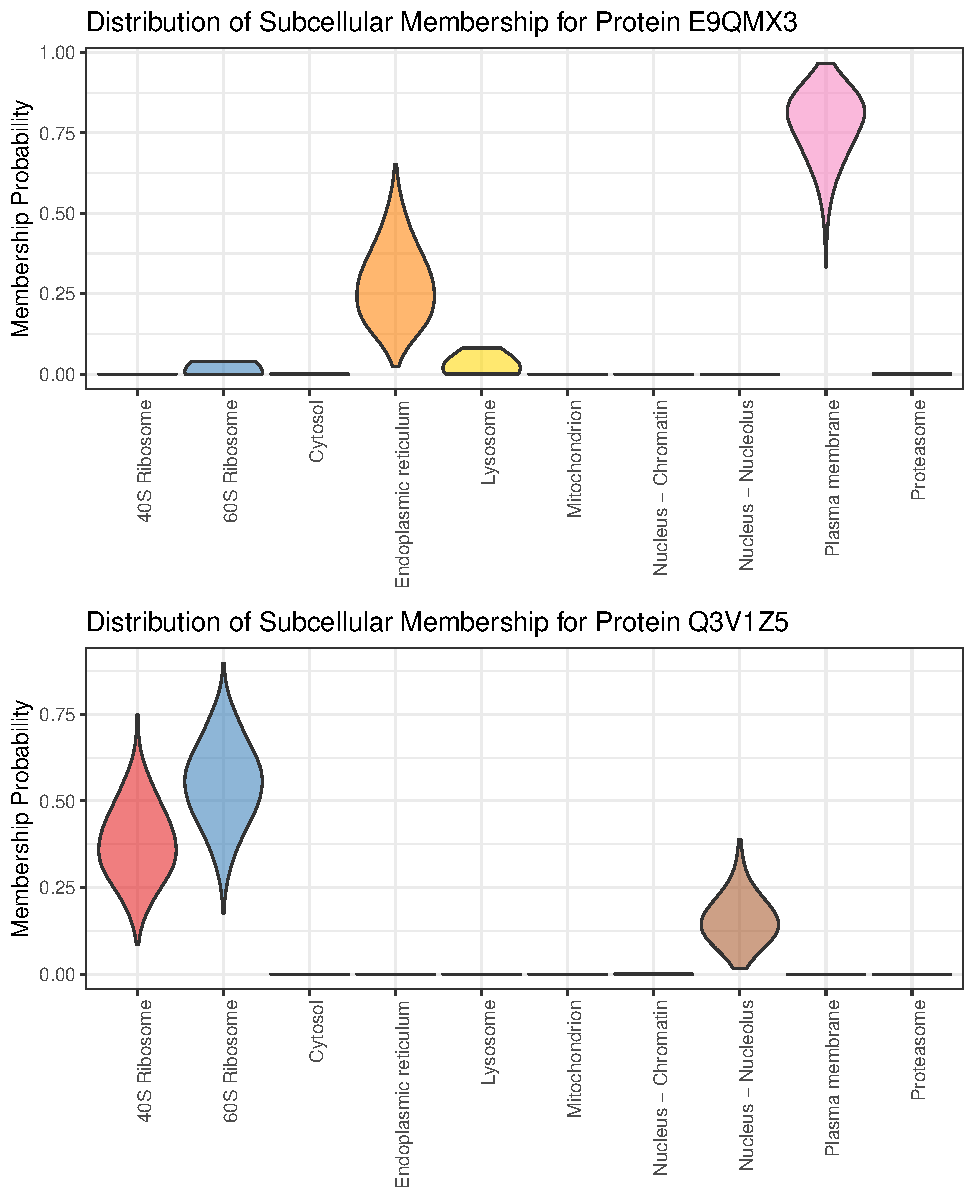
\includegraphics{F1000TAGMworkflow_files/figure-latex/probdists1-1} 

}

\caption{Full posterior distribution of localisation probabilities for individual proteins.}\label{fig:probdists1}
\end{figure}

\hypertarget{discussion}{%
\section{Discussion}\label{discussion}}

The Bayesian analysis of biological data is of clear interest to many
because of its ability to provide richer information about the
experimental results. A fully Bayesian analysis differs from other
machine learning approaches, since it can quantify the uncertainty in
our inferences. Furthermore, we use a generative model to explicitly
describe the data, which makes inferences more interpretable compared to
the less interpretable outputs of black-box classifiers such as, for
example, support vector machines (SVM).

Bayesian analysis is often characterised by its provision of a (posterior)
probability distribution over the biological parameters of interest, as opposed
to single point estimate of these parameters. In the case that is presented in this workflow,
a Bayesian analysis ``computes'' a posterior probability distribution over the
protein localisation probabilities. These probability distributions can then be
rigorously interrogated for greater biological insight; in addition, it may
allow us to ask additional questions about the data, such as whether a protein
might be multi-localised.

Despite the wealth of information a Bayesian analysis can provide, the uptake
amongst cell biologists is still low. This is because a Bayesian analysis
presents a new set of challenges and little practical guidance exists regarding how to address these challenges.
Bayesian analyses often rely on computatinally intensive approaches such as Markov-chain Monte-Carlo
(MCMC) and a practical understanding of these algorithms and the interpretation of their
output is a key barrier to their use. A Bayesian analysis usually consists of three
broad steps: (1) Data pre-processing and algorithmic implementation,
(2) assessing algorithmic convergence and (3) summarising and visualising the results.
This workflow provides a set of tools to simplify these steps and provides
step-by-step guidance in the context of the analysis of spatial proteomics data.

We have provided a workflow for the Bayesian analysis of spatial
proteomics using the \texttt{pRoloc} and \texttt{MSnbase} software. We have
demonstrated, in a step-by-step fashion, the challenges and advantages
associated with taking a Bayesian approach to data analysis. We hope this workflow
will help spatial proteomics practitioners to apply our methods and
will motivate others to create detailed documentation for the Bayesian
analysis of biological data.

\hypertarget{session-information}{%
\section{Session information}\label{session-information}}

Below, we provide a summary of all packages and versions used to
generate this document.

\begin{Shaded}
\begin{Highlighting}[]
\KeywordTok{sessionInfo}\NormalTok{()}
\end{Highlighting}
\end{Shaded}

\begin{verbatim}
## R version 3.5.2 Patched (2019-01-24 r76018)
## Platform: x86_64-pc-linux-gnu (64-bit)
## Running under: Manjaro Linux
## 
## Matrix products: default
## BLAS: /usr/lib/libblas.so.3.8.0
## LAPACK: /usr/lib/liblapack.so.3.8.0
## 
## locale:
##  [1] LC_CTYPE=en_US.UTF-8       LC_NUMERIC=C              
##  [3] LC_TIME=en_US.UTF-8        LC_COLLATE=en_US.UTF-8    
##  [5] LC_MONETARY=en_US.UTF-8    LC_MESSAGES=en_US.UTF-8   
##  [7] LC_PAPER=en_US.UTF-8       LC_NAME=C                 
##  [9] LC_ADDRESS=C               LC_TELEPHONE=C            
## [11] LC_MEASUREMENT=en_US.UTF-8 LC_IDENTIFICATION=C       
## 
## attached base packages:
## [1] stats4    parallel  stats     graphics  grDevices utils     datasets 
## [8] methods   base     
## 
## other attached packages:
##  [1] patchwork_0.0.1      pRolocdata_1.21.1    pRoloc_1.23.2       
##  [4] coda_0.19-2          mixtools_1.1.0       BiocParallel_1.16.6 
##  [7] MLInterfaces_1.62.0  cluster_2.0.7-1      annotate_1.60.1     
## [10] XML_3.98-1.19        AnnotationDbi_1.44.0 IRanges_2.16.0      
## [13] MSnbase_2.9.3        ProtGenerics_1.14.0  S4Vectors_0.20.1    
## [16] mzR_2.17.2           Rcpp_1.0.0           Biobase_2.42.0      
## [19] BiocGenerics_0.28.0 
## 
## loaded via a namespace (and not attached):
##   [1] tidyselect_0.2.5        RSQLite_2.1.1          
##   [3] htmlwidgets_1.3         grid_3.5.2             
##   [5] trimcluster_0.1-2.1     lpSolve_5.6.13         
##   [7] rda_1.0.2-2.1           devtools_2.0.1         
##   [9] munsell_0.5.0           codetools_0.2-16       
##  [11] preprocessCore_1.44.0   withr_2.1.2            
##  [13] colorspace_1.4-0        knitr_1.22             
##  [15] rstudioapi_0.9.0        robustbase_0.93-3      
##  [17] mzID_1.20.1             labeling_0.3           
##  [19] git2r_0.24.0            hwriter_1.3.2          
##  [21] bit64_0.9-7             ggvis_0.4.4            
##  [23] rprojroot_1.3-2         generics_0.0.2         
##  [25] ipred_0.9-8             xfun_0.5               
##  [27] randomForest_4.6-14     diptest_0.75-7         
##  [29] R6_2.4.0                doParallel_1.0.14      
##  [31] flexmix_2.3-15          bitops_1.0-6           
##  [33] assertthat_0.2.0        promises_1.0.1         
##  [35] scales_1.0.0            nnet_7.3-12            
##  [37] gtable_0.2.0            affy_1.60.0            
##  [39] processx_3.3.0          timeDate_3043.102      
##  [41] rlang_0.3.1             genefilter_1.64.0      
##  [43] splines_3.5.2           lazyeval_0.2.1         
##  [45] ModelMetrics_1.2.2      impute_1.56.0          
##  [47] hexbin_1.27.2           BiocManager_1.30.4     
##  [49] yaml_2.2.0              reshape2_1.4.3         
##  [51] threejs_0.3.1           crosstalk_1.0.0        
##  [53] backports_1.1.3         httpuv_1.4.5.1         
##  [55] caret_6.0-81            tools_3.5.2            
##  [57] lava_1.6.5              usethis_1.4.0          
##  [59] bookdown_0.9            ggplot2_3.1.0          
##  [61] affyio_1.52.0           RColorBrewer_1.1-2     
##  [63] proxy_0.4-23            sessioninfo_1.1.1      
##  [65] plyr_1.8.4              base64enc_0.1-3        
##  [67] progress_1.2.0          zlibbioc_1.28.0        
##  [69] purrr_0.3.1             RCurl_1.95-4.12        
##  [71] ps_1.3.0                prettyunits_1.0.2      
##  [73] rpart_4.1-13            viridis_0.5.1          
##  [75] sampling_2.8            sfsmisc_1.1-3          
##  [77] LaplacesDemon_16.1.1    fs_1.2.6               
##  [79] magrittr_1.5            data.table_1.12.0      
##  [81] pcaMethods_1.74.0       mvtnorm_1.0-10         
##  [83] whisker_0.3-2           pkgload_1.0.2          
##  [85] hms_0.4.2               mime_0.6               
##  [87] evaluate_0.13           xtable_1.8-3           
##  [89] mclust_5.4.2            gridExtra_2.3          
##  [91] testthat_2.0.1          compiler_3.5.2         
##  [93] biomaRt_2.38.0          tibble_2.0.1           
##  [95] ncdf4_1.16.1            crayon_1.3.4           
##  [97] htmltools_0.3.6         segmented_0.5-3.0      
##  [99] later_0.8.0             BiocWorkflowTools_1.8.0
##  [ reached getOption("max.print") -- omitted 49 entries ]
\end{verbatim}

The source of this document, including the code necessary to reproduce
the analyses and figures is available in a public manuscript
repository on GitHub \citep{ghrepo}.

\hypertarget{competing-interests}{%
\section{Competing interests}\label{competing-interests}}

No competing interests were disclosed.

\hypertarget{grant-information}{%
\section{Grant information}\label{grant-information}}

PDWK was supported by the MRC (project reference MC\_UU\_00002/10). LMB
was supported by a BSRC Tools and Resources Development grant (Award
BB/N023129/1) and a Wellcome Trust Technology Development Grant (Grant
number 108441/Z/15/Z). OMC is a Wellcome Trust Mathematical Genomics
and Medicine student supported financially by the School of Clinical
Medicine, University of Cambridge. The funders had no role in study
design, data collection and analysis, decision to publish, or
preparation of the manuscript.

\renewcommand\refname{References}
{\small\bibliography{BayesProt.bib}}

\end{document}
